\documentclass[online]{jfp}

% jfp.cls uses newtxmath which defines \Bbbk, but amssymb also defines \Bbbk
\let\Bbbk\relax

\usepackage{amssymb}
\usepackage{amsfonts}
\usepackage{mathtools}
\usepackage{stmaryrd}
\usepackage{minted}
\usepackage{mathpartir}
\usepackage{xspace}
\usepackage[shortcuts]{extdash}
\usepackage{enumitem}
\usepackage[title]{appendix}
\usepackage{proof}
\usepackage{suffix}
\usepackage{ifthen}
\usepackage{multicol}
\usepackage{stackengine}
\usepackage[skip=5pt, belowskip=-6pt]{caption}
\usepackage{pstc}

\def\sectionautorefname{Section}
\def\subsectionautorefname{Subsection}
\def\subsubsectionautorefname{Subsubsection}
\def\figureautorefname{Figure}
\def\tableautorefname{Table}
\def\Appendixautorefname{Appendix}

\newtheorem{theorem}{Theorem}[section]
\newtheorem{definition}[theorem]{Definition}
\newtheorem{conjecture}[theorem]{Conjecture}

\newmintinline[coqinline]{coq}{escapeinside=<>,mathescape=true}

\begin{document}

\journaltitle{JFP}
\cpr{Cambridge University Press}
\doival{10.1017/42069}
\totalpg{\pageref{lastpage}}
\jnlDoiYr{2021}

% To reconsider
%\title{Practical Sized Typing for Coq}
\title{Is Sized Typing for Coq Practical?}

\begin{authgrp}
  \author{Jonathan Chan}
  \affiliation{
    University of British Columbia\\
    \emaillink{jcxz@cs.ubc.ca}
  }
  \author{Yufeng Li}
  \affiliation{
    University of Waterloo\\
    \emaillink{yufeng.li@uwaterloo.ca}
  }
  \author{William J. Bowman}
  \affiliation{
    University of British Columbia\\
    \emaillink{wjb@williamjbowman.com}
  }
\end{authgrp}

\begin{abstract}
Contemporary proof assistants such as Coq require that recursive functions be terminating and corecursive functions be productive to maintain logical consistency of their type theories,
and some ensure these properties using syntactic checks.
However, being syntactic, they are inherently delicate and restrictive,
preventing users from easily writing obviously terminating or productive functions at its whim.

Meanwhile, there exist many \emph{sized type theories} that perform type-based termination and productivity checking,
including theories based on the Calculus of (Co)Inductive Constructions (CIC), the core calculus underlying Coq.
These theories are more robust and compositional in comparison.
So why haven't they been adapted to Coq?

In this paper, we venture to answer this question with \lang, a sized type theory based on CIC.
It extends past work on sized types in CIC with additional Coq features such as global and local definitions.
We also present a corresponding size inference algorithm and implement it within Coq's kernel;
for maximal backward compatibility with existing Coq developments,
it requires no additional annotations from the user.

In our evaluation of the implementation, we find a severe performance degredation when compiling parts of the Coq standard library, inherent to the algorithm itself.
We conclude that if we wish to maintain backward compatibility,
using size inference as a replacement for syntactic checking is wildly impractical in terms of performance.

\iffalse
Termination of recursive functions and productivity of corecursive functions are important for maintaining logical consistency in proof assistants.
However, contemporary proof assistants, such as Coq, rely on fragile syntactic criteria that prevent users from easily writing some obviously terminating or productive functions.
This is troublesome, as there exist theories for type-based termination and productivity checking.

In this paper, we present a design and implementation of sized type checking and inference for Coq.
We extend past work on sized types for the Calculus of (Co)Inductive Constructions (CIC) to support definitions, and extend the sized type inference algorithm to support completely unannotated CIC terms.
This allows our design to maintain complete backward compatibility with existing Coq developments.
We provide an implementation that extends the Coq kernel with optional support for sized types.
\fi
\end{abstract}

%%% Local Variables:
%%% TeX-master: "../main.tex"
%%% TeX-engine: default
%%% End:


\maketitle
%\tableofcontents

\section{Introduction}\label{sec:intro}

Proof assistants based on dependent type theory rely on the termination of recursive functions and the productivity of corecursive functions to ensure two important properties: logical consistency, so that it is not possible to prove false propositions; and decidability of type checking, so that checking that a program proves a given proposition is decidable.

In proof assistants such a Coq, termination and productivity are enforced by a \emph{guard predicate} on fixpoints and cofixpoints respectively.
For fixpoints, recursive calls must be \emph{guarded by destructors}; that is, they must be performed on structurally smaller arguments.
For cofixpoints, corecursive calls must be \emph{guarded by constructors}; that is, they must be the structural arguments of a constructor.
The following examples illustrate these structural conditions.

\begin{samepage}
\begin{minted}{coq}
Fixpoint plus n m : nat :=
  match n with
  | O => m
  | S p => S (plus p m)
  end.
Variable A : Type.
CoFixpoint const a : Stream A := Cons a (const a).
\end{minted}
\end{samepage}

In the recursive call to \coqinline{plus}, the first argument \coqinline{p} is structurally smaller than \coqinline{S p}, which is the form of the original first argument \coqinline{n}. Similarly, in \coqinline{const}, the constructor \coqinline{Cons} is applied to the corecursive call.

The actual implementation of the guard predicate extends beyond the \guardedbydestructors and \guardedbyconstructors conditions to accept a larger set of terminating and productive functions.
In particular, function calls will be unfolded (\ie inlined) in the bodies of \cofixpoints as needed before checking the guard predicate.
This has a few disadvantages: firstly, the bodies of these functions are required, which hinders modular design; and secondly, the \cofixpoint bodies may become very large after unfolding, which can decrease the performance of type checking.

Furthermore, changes in the structural form of functions used in \cofixpoints can cause the guard predicate to reject the program even if the functions still behave the same.
The following simple example, while artificial, illustrates this structural fragility.
\begin{minted}{coq}
Fixpoint minus n m :=
  match n, m with
  | O, _ => n
  | _, O => n
  | S n', S m' => minus n' m'
  end.
\end{minted}
\begin{minted}{coq}
Fixpoint div n m :=
  match n with
  | O => O
  | S n' => S (div (minus n' m) m)
  end.
\end{minted}

If we replace \coqinline{| O, _ => n} with \coqinline{| O, _ => O} in \coqinline{minus}, the behaviour does not change, but \coqinline{O} is not a structurally smaller term of \coqinline{n} in the recursive call to \coqinline{div}, so \coqinline{div} no longer satisfies the guard predicate.
The acceptance of \coqinline{div} then depends on a function external to it, which can lead to difficulty in debugging for larger programs.
Furthermore, the guard predicate is unaware of the obvious fact that \coqinline{minus} never returns a \coqinline{nat} larger than its first argument, which the user would have to prove in order for \coqinline{div} to be accepted with our alternate definition of \coqinline{minus}.

In short, the syntactic guard condition long used by Coq is anti-modular, anti-compositional, has poor performance characteristics, and requires the programmer to either avoid certain algorithms to pay large cost in proof burden.

This situation is particularly unfortunate, as the Agda programmer is aware, given that there exists a non-syntactic termination and productivity condition which solves essentially all of these problems, whose theory has existed for nearly as long as the guard condition---\emph{sized types}!

In essence, the \coinductive type of an object is annotated with a size annotation, which provides some information about the size of the object.
In this paper, we consider a simple size algebra: \mbox{$s \coloneqq \upsilon \mid \hat{s} \mid \infty$}, where $\upsilon$ ranges over size variables.
If the argument to a constructor has size $s$, then the fully-applied constructor would have a successor size $\hat{s}$.
For instance, the constructors for the naturals follow the below rules:

\vspace{-2ex}
\begin{mathpar}
  \inferrule*
    {~}
    {\Gamma \vdash \Zero : \Nat^{\hat{s}}}
  \and
  \inferrule*
    {\Gamma \vdash n : \Nat^s}
    {\Gamma \vdash \app{\Succ}{n} : \Nat^{\hat{s}}}
\end{mathpar}

Termination and productivity checking is then \emph{just} a type checking rule that uses size information.
For termination, the recursive call must be done on an object with a smaller size, so when typing the body of the fixpoint, the reference to itself in the typing context must have a smaller size.
For productivity, the returned object must have a larger size than that of the corecursive call, so the type of the body of the cofixpoint must be larger than the type of the reference to itself in the typing context.
In short, they both follow the following (simplified) typing rule, where $\upsilon$ is an arbitrary fresh size variable annotated on the inductive types, and $s$ is an arbitrary size expression as needed.

\vspace{-2ex}
\begin{mathpar}
  \inferrule*[]
    {\Gamma (\assm{f}{t^\upsilon}) \vdash e: t^{\hat{\upsilon}}}
    {\Gamma \vdash \kw{(co)fix}\ f \mathbin{:} t \mathbin{\coloneqq} e : t^s}
\end{mathpar}

We can then assign \coqinline{minus} the type $\text{Nat}^\iota \to \text{Nat} \to \text{Nat}^\iota$.
The fact that we can assign it a type indicates that it will terminate, and the $\iota$ annotations indicate that the function preserves the size of its first argument.
Then \coqinline{div} uses only the type of \coqinline{minus} to successfully type check, not requiring its body.
Furthermore, being type-based and not syntax-based, replacing \coqinline{| O, _ => n} with \coqinline{| O, _ => O} does not affect the type of \coqinline{minus} or the typeability of \coqinline{div}.
Similarly, some other \cofixpoints that preserve the size of arguments in ways that aren't syntactically obvious may be typed to be size preserving, expanding the set of terminating and productive functions that can be accepted.
Finally, if additional expressivity is needed, rather than syntactic hacks like inlining, we can take the semantic approach of enriching the size algebra.

It seems perfect; so why doesn't Coq \emph{just} use sized types?

That is the question we seek to answer in this paper.

Unfortunately, past work on sized types~\citep{cic-hat, cic-hat-minus} in the Calculus of (Co)\-Inductive Constructions (CIC), Coq's underlying calculus, have some practical issues:

\begin{itemize}
    \item They require nontrivial backwards-incompatible additions to the surface language.
      These include annotations that mark the positions of \corecursive and size-preserved types, and polarity annotations on \coinductive definitions that describe how subtyping works with respect to parameters.
    \item They require the \corecursive arguments of \cofixpoints to have literal \coinductive types.
      That is, the types cannot be expressions that convert to \coinductive types.
    \item Their languages do not support local and global definitions, which Coq includes.
%      In particular, size inference should be done locally, \ie confined to within a single global definition.
\end{itemize}

We start by solving these theoretical problems.
We design \lang (``\emph{CIC-star-hat}''), a calculus for representing the core of Coq with sized types, and an inference algorithm from CIC to \lang.
It is an extension of \CIChat~\citep{cic-hat} and \CIChatminus~\citep{cic-hat-minus} that resolves the issues above.
We prove subject reduction, confluence, and strong normalization of a subset of \lang including W types.

However, in attempting to recover backwards-compatibility and the entire feature set of Coq, we run into new theoretical problems.
Proving strong normalization and consistency of the new language becomes difficult compared to pure CIC, for reasons that seem intrinsic.
Some of the design goals of CIC---untyped reduction, orthogonality to classical axioms---seem at odds with set theoretical models that include sized types.
Some of these might be solvable if we could sacrifice backwards compatibility.
Even if they are solvable, the complexity of these models would at least sacrifice trust in the core of Coq.
We discuss our models and the meta-theory of \lang in detail.

We then ask a second question: even supposing we can solve the theoretical problems and finish the proof of strong normalization and consistency, is the implementation of this system practical?
We have forked Coq\blindimpl\xspace and implemented the size inference algorithm and size-based termination and productivity checking of \lang.
To maximize backward compatibility, the surface language is completely unchanged, and the existing guard condition and sized types can be enabled or disabled independently, or used in conjunction.
Sized typing can be turned on with a flag that is off by default for safe and gradual testing of the new kernel.
\blinding{We are currently working with the Coq development team to merge the work into Coq.}{A draft pull request in the Coq repository has been opened for this fork.\footnote{\url{https://github.com/coq/coq/pull/12426/}}}

While the sized typing enables many of our goals, namely increased expressivity with modular and compositional typing for \cofixpoints, the performance cost is unacceptable.
We measure at least 16x increase in compilation time in some standard libraries.
The performance cost seems to be intrinsic to the size inference algorithm, and thus, intrinsic to attempting to maintain backwards compatibility.
We analyze the performance of our size inference algorithm, and our implementation in detail.

The short answer to our question, ``why doesn't Coq \emph{just} use sized types'', seems to be that Coq must either sacrifice backwards compatibility, some of its syntactic meta-theory, and/or compile time performance to do so.
While this isn't possible, it seems wildly impractical.

The remainder of this paper is organized as follows.
We begin in \autoref{sec:sponge-cake} with a high-level overview of the design of \lang, its role in Coq, and the main lessons from our design.
We formalize the calculus \lang in \autoref{sec:typing}.
In \autoref{sec:algorithm}, we present a size inference algorithm from CIC terms to sized \lang terms that details how we annotate the types of \cofixpoints, how we deal with the lack of polarities, and how definitions are supported, and termination and productivity checking.
% In \autoref{sec:examples}, we provide a few examples of programs that pass sized typing but not guard checking and vice versa, discuss some categories of terminating programs that cannot be typed in \lang, and step through the size inference algorithm for an example program.
\autoref{sec:metatheory} states some of the metatheoretical properties of \lang that have been proven or remain to be proven.
Finally, we briefly compare with the past work on sized types for CIC and related languages in \autoref{sec:related}.

%%% Local Variables:
%%% TeX-master: "../main.tex"
%%% TeX-engine: default
%%% End:

\section{Overview}\label{sec:overview} % Time for a facelift

As mentioned, \lang is an extension of \CIChat and \CIChatminus.
These add sized types to CIC with the explicit philosophy of requiring no size annotations:
a user would write bare CIC code, and the type checker would have the simultaneous task of inferring all the size annotations.
However, Coq's core calculus extends quite a bit beyond merely CIC,
and the presentation of various analogous features differ subtly but nontrivially.
The goal of \lang is to bring sized types in CIC a few steps closer to Coq,
while keeping with the original philosphy.
In the process of conforming to Coq's calculus, to minimize the changes required to it so that a prototype implementation is viable --- for Coq's codebase itself is old, large, fragile, and intricate --- we must also discard some features from \CIChatminus.
In this section, we discuss what \lang has added or removed relative to past work and to Coq,
and their implications on the metatheory and the implementation.

\subsection{Definitions}

Coq's core calculus contains two types of variables:%
\footnote{It also has a third type of variable for section-level bindings;
this is beyond the scope of \lang.}
one for local bindings from functions, function types, and let expressions,
and one for global bindings from vernacular declarations such as \coqinline{Definition} and \coqinline{Parameter} (which we call \textit{constants}).
\lang adds let expressions and global declarations to \CIChatminus,
with separate local and global environments,
and definitions in the environments in the style of a PTS with definitions~\citep{ptsdef}.

Gobal definitions and let expressions let us define aliases for types for concision and organization of code,
which necessitates a form of size polymorphism if we want the aliases to behave as we expect.
For instance, if we globally define $\Defn{N}{\Type{}}{\Nat^\upsilon}$,
and later want to define an addition function with type $N \rightarrow N \rightarrow N$,
it would \emph{not} be correct to perform the na\"ive substitution to get $\Nat^\upsilon \rightarrow \Nat^\upsilon \rightarrow \Nat^\upsilon$:
addition intuitively does not always return something of the same size.

What we want instead is to allow a different size for each use of $N$,
allowing the above type to reduce to $\Nat^{\upsilon_1} \rightarrow \Nat^{\upsilon_2} \rightarrow \Nat^{\upsilon_3}$.
This means $N$ must be polymorphic in the sizes involved in its definition,
the same kind of rank-1 or prenex polymorphism in ML-style let polymorphism for type variables.
To retain backward compatibility, there is no explicit size quantification ---
every definition and let binding is implicitly quantified over \emph{all} size variables involved.
The corresponding notion of size instantiation comes in the form of size annotations on variables and constants, so that $N^s$ for instance reduces to $\Nat^s$.
These and all other size annotations are inferrable, as detailed in \autoref{sec:algorithm}.

Having definitions and annotated variables and constants also means we need to allow sizes to appear
not only in the bodies of let expressions but also in the bodies of functions and in the branches of case expressions,
in contrast to \CIChatminus.
% TODO: Ask Michael about the consequences of this on normalization.

\paragraph*{} While \CIChat's size inference algorithm takes a local environment and an unannotated term
and returns a size-annotate term and its type along with a set of constraints on their size annotations,
we need to handle inference of global declarations.
Left with a constraint set after inference of a definition's body, we have two options:
attach the constraints to the definition in the environment,
or ``solve'' the constraints by reassigning size variables with sizes that satisfy those constraints.
Global definitions in Coq are relatively independent in terms of type checking,
so we choose the second option for its modularity:
constraints derived from previous definitions should not interfere with the size inference of the current definition.
On the other hand, to reduce the overhead of solving constraints,
we choose the first option for local definitions.
The way constraints are added to the environment is inspired by \citet{universes},
which infers universe levels that are prenex polymorphic at definitions.

Unfortunately, even when only solving constraints for global declarations,
our implementation of the size inference algorithm in the Coq codebase takes a rather significant performance hit.
This is in part due to the proliferation of sizes that definitions are polymorphic over,
as the worst-case time complexity of solving is quadratic in the number of size variables.
We analyze the performance of our implementation and possible causes and solutions in a subsequent section.
% TODO: Add an autoref to the right section once it exists.

\subsection{Polarities}

% mention effects on nested inductives/subject reduction

\subsection{Restrictions on Type Annotations}

% why we can't have simple types
% why constructors can't have erased parameters
% why (co)fixpoint types need to be terms in general

\subsection{Position Size Annotations}

% these are the star annotations on (co)fixpoint types
% this is why we need RecCheckLoop on top of RecCheck
% it's okay though. it's just like how Coq finds the recursive arg by trying each one

\subsection{Universes}

% we add cumulativity but NOT polymorphism
% we add impredicative Prop but NOT strict Prop
% these have effects on the metatheory. ask Michael

\section{Overview}\label{sec:sponge-cake}
Our goal in the design of \lang is to balance backward compatibility with performance.
We could achieve backward compatibility easily by \emph{just} using an extremely expressive size algebra, but we could never implement an efficient type checker.
Similarly, we could easily add sized types to Coq with efficient checking if we \emph{just} make the users and the Coq developers rewrite all their code in our cool new annotated language.
Both of these are impractical.
Instead, we try to thread the needle.

Our first design decision is complete backward compatibility: the Coq user must not be required to provide new annotations on existing code, and ideally should be able to get the advantages of sized typing in all new code.
If we expect the user to reuse any standard library data types with sized types, this means that we need a \emph{size inference} algorithm, which takes ordinary Coq programs, infers size annotations as needed, uses sizes during type checking, and returns ordinary Coq programs.

For performance, we want size inference to be local --- size variables and constraints should be independent from one global declaration to another.
In theory, we have an infinite set of unique size variables that can be summoned at will, but in practice, each variable needs to be generated and tracked, consuming time and space.
Similarly, we could add an unrestricted number of constraints, but as we discuss in \autoref{sec:algorithm}, the time complexity of size inference is proportional to the number of constraints.
By keeping size inference local, the state of size information and size constraint sets can be kept smaller.

Below is a high-level view of our type checking process.
The pipeline is local, \ie each top-level definition in a Coq program is run through this pipeline in turn.
\begin{equation*}
  \text{CIC} \equiv \text{bare \lang} \xrightarrow{\text{inference}} \text{sized \lang} \xrightarrow{\text{erasure}} \text{limit \lang}
\end{equation*}

The first pass elaborates Coq code into a fully type-annotated CIC term.
This is a standard pass for Coq which we will not discuss further.
Naturally, the CIC term will have no size annotations; we also call this \emph{bare} \lang.

Next, we perform size inference on bare \lang to obtain \emph{sized} \lang.
There are three different tasks in size inference: (1) annotate all \coinductive types with fresh size variables; (2) during type checking, whenever two terms are compared, follow subtyping rules to generate a set of constraints between their size annotations; and (3) when type checking a \cofixpoint, check that the collected constraints are satisfiable.
By representing the constraints as a weighted directed graph, this amounts to checking for negative cycles.

The final step in the pipeline is to erase unnecessary size annotations from sized \lang to obtain \emph{limit} \lang by replacing size annotations with $\infty$.
This is the same strategy adopted in a prototype implementation of \CIChatminus~\citep{cicminus}.

However, not all size annotations are erased.
We preserve annotations for each \emph{size-preserving} \corecursive function, which is a key feature of \lang that enables additional expressiveness in termination and productivity checking.
Consider, for example, an inductive list of type $\text{List}^r ~ A$ and a coinductive stream of type $\text{Stream}^s ~ A$.
The intuitive notion of the size $r$ is the length of the list.
Since every list of $A$s is an inhabitant of $\text{List}^\infty ~ A$, we can imagine that the inhabitants of $\text{List}^r ~ A$ are lists of length $r$ or shorter.
Dually, the inhabitants of $\text{Stream}^s ~ A$ are streams of ``length'' $s$ or ``longer''.
From the perspective of productivity, these are streams that can produce at least $s$ elements.
A recursive function on lists that is size-preserving, then, is one that returns a list of equal or smaller size, while a size-preserving corecursive function on streams is one that returns a stream of equal or larger size.
For instance, a \texttt{map} function over lists or streams is size-preserving, since it does not modify their lengths.
Whether a \corecursive function is size-preserving or not is determined during the size inference step, which annotates the types of \cofixpoints with position annotations $*$ to mark the \corecursive argument type as well as any size-preserving return types.
These annotations are not erased.

This alone is not enough to express size-preservation of global declarations.
A globally-defined \cofixpoint is annotated with the \emph{definition}'s type, which doesn't expose the size-preservedness expressed by the \emph{\cofixpoint}'s type.
Therefore, we also annotate the types of such definitions with global annotations $\iota$ to mark what would have been position annotations.

The examples \coqinline{filter} and \coqinline{qsort} below demonstrate what limit \lang programs look like after erasure.
During the inference step for \coqinline{qsort}, the global annotations on \coqinline{filter} are substituted by the \textit{same} size variable, which tells \coqinline{qsort} that \coqinline{filter} preserves the size of the recursive argument, allowing us to use it in the recursive call.
Global annotations then are essentially a limited form of size polymorphism with one universal quantifier, which is sufficient to express size preservation.

\begin{multicols}{2}
\begin{minted}[escapeinside=<>,mathescape=true]{coq}
Def filter: (Nat<$^\infty$> <$\rightarrow$> Bool<$^\infty$>) <$\rightarrow$>
  List<$^\iota$> Nat<$^\infty$> <$\rightarrow$> List<$^\iota$> Nat<$^\infty$> <$\coloneqq$>
  fix filter': (Nat <$\rightarrow$> Bool) <$\rightarrow$>
    List<$^*$> Nat <$\rightarrow$> List<$^*$> Nat <$\coloneqq$>
    <$\lambda$>p: Nat <$\rightarrow$> Bool. <$\lambda$>l: List Nat.
    case l return List Nat of
    | Nil <$\Rightarrow$> Nil
    | Cons <$\Rightarrow$> <$\lambda$>hd: Nat. <$\lambda$>tl: List Nat.
      if p hd
      then Cons Nat hd (filter' p tl)
      else (filter' p tl)
    end.
(* [append], [gtb], [leb] omitted *)
Def qsort: List<$^\iota$> Nat<$^\infty$> <$\rightarrow$> List<$^\infty$> Nat<$^\infty$> <$\coloneqq$>
  fix qsort': List<$^*$> Nat <$\rightarrow$>
    List Nat <$\coloneqq$> <$\lambda$>l : List Nat.
    case l return List Nat of
    | Nil <$\Rightarrow$> Nil
    | Cons <$\Rightarrow$> <$\lambda$>hd: Nat. <$\lambda$>tl: List Nat.
      append
      (qsort' (filter (gtb hd) tl))
      (Cons Nat hd
        (qsort' (filter (leb hd) tl)))
    end.
\end{minted}
\end{multicols}

There is a second problem with erasure.
Consider the following \lang program.

\begin{minted}[escapeinside=<>,mathescape=true]{coq}
  Def N: Type <$\coloneqq$> Nat<$^\infty$>.
  Def add: N<$^\iota$> <$\rightarrow$> N <$\rightarrow$> N <$\coloneqq$>
    let id: N <$\rightarrow$> N <$\coloneqq$> <$\lambda$>n: N. n in
    fix add': N<$^*$> <$\rightarrow$> N <$\rightarrow$> N <$\coloneqq$> <$\lambda$>n: N. <$\lambda$>m: N.
      case n return N of
      | O <$\Rightarrow$> m
      | S <$\Rightarrow$> <$\lambda$>n': N. S (add' (id n') m)
      end.
\end{minted}

\coqinline{N} will reduce to \coqinline{Nat} during type checking, but what size should \coqinline{Nat} then have?
It cannot have the limit size $\infty$ left after erasure; this would disallow us from using \coqinline{id} in the recursive call to \coqinline{add'}, since termination checking requires that \coqinline{id} preserve the size of \coqinline{n'} and not return some \emph{larger} \coqinline{Nat<$^\infty$>}.
However, we cannot \textit{not} erase, either, leaving \coqinline{Nat} with some arbitrary fixed size annotation, since this makes \coqinline{add}'s type size-preserving when \coqinline{add} is not.
To handle this example, each instance of \coqinline{N} should have its own fresh size annotation; during reduction, this becomes a size-annotated \coqinline{Nat}.

We support this kind of program in \lang by treating global definitions essentially as implicitly abstracting over size expressions.
Each instance of a variable bound to a definition needs to be instantiated with the correct number of size expressions, and so carries a vector of size expressions whose length is the number of $\infty$ annotations in the body after erasure.
Like size annotations, these new vector annotations are only found in sized \lang.

A final design decision remains to enable backward compatibility.
Our sized typing enables many new programs to type check easily, such as \coqinline{qsort} above, but our limited sized algebra means that there also exist programs that pass guard checking but not our sized typing pipeline.
Guard checking unfolds definitions, which is bad for modularity and performance, but enables \texttt{gcd} as defined in the Coq standard library to type check using guard checking.
On the other hand, \texttt{gcd} cannot be type checked using sized types with our size algebra\footnote{\url{https://github.com/coq/coq/wiki/CoqTerminationDiscussion\#sized}}.
We could enrich the size algebra, but as we discuss in \autoref{sec:related}, this greatly increases the time complexity of size inference.
To take advantage of both schemas, our implementation enables each to be used simultaneously, so the type checker accepts a program if it passes either sized typing \textit{or} guard checking:

\begin{minted}{coq}
Set Guard Checking. Set Sized Typing.
\end{minted}

%%% Local Variables:
%%% TeX-master: "../main.tex"
%%% TeX-engine: default
%%% End:

\section{\titlelang}\label{sec:typing}
In this section, we present \lang, a core calculus for sized typing in Coq.

\subsection{Syntax}

%We use the overline $\overline{\,\cdot\,}$ to denote a sequence of some construction.
%For instance, $\overline{\mathcal{V}}$ is a sequence of size variables $\mathcal{V} \dots \mathcal{V}$.

\begin{figure}
\centering
\begin{align*}
S &\Coloneqq \mathcal{V} \mid \mathcal{V}^* \mid \succ{S} \mid \infty &\text{size expressions} \\
U &\Coloneqq \text{Prop} \mid \text{Set} \mid \text{Type}_n &\text{set of universes}
\end{align*}
\begin{align*}
T[\alpha] &\Coloneqq \\
    &\mid U
        &\textit{universes}\\
    &\mid \mathcal{X} \mid \mathcal{X}^{\seq{\alpha}}
        &\textit{variables} \\
    &\mid \abs{\mathcal{X}}{T^\circ\!}{T[\alpha]}
        &\textit{abstractions} \\
    &\mid T[\alpha] T[\alpha]
        &\textit{applications} \\
    &\mid \prod{\mathcal{X}}{T[\alpha]}{T[\alpha]}
        &\textit{function types} \\
    &\mid \text{let} ~ \mathcal{X} : T^\circ \coloneqq T[\alpha]  ~ \text{in} ~ T[\alpha]
        &\textit{let expressions} \\
    &\mid \mathcal{I}^\alpha
        &\textit{(co)inductive types} \\
    &\mid \mathcal{C}
        &\textit{(co)ind. constructors} \\
    &\mid \text{case}_{T^\circ}  ~ T[\alpha]  ~ \text{of}  ~ \seq{\mathcal{C} \Rightarrow T[\alpha]}
        &\textit{case expressions} \\
    &\mid \text{fix}_{\seq{n}, m}  ~ \seq{\mathcal{X}: T^* \coloneqq T[\alpha]}
        &\textit{fixpoints} \\
    &\mid \text{cofix}_{m}  ~ \seq{\mathcal{X}: T^* \coloneqq T[\alpha]}
        &\textit{cofixpoints}
\end{align*}
\caption{Syntax of \lang terms with annotations $\alpha$}
\label{fig:terms-general}
\end{figure}


\autoref{fig:terms-general} presents the syntax of \lang,
with distinct size and term variables as well as \coinductive type names and \coinductive constructor names,
and terms $e$ annotated with size expressions $s$.
We use $m$ and $n$ as well as $i, j, k, \ell$ as metavariables for positive naturals used in indexing; note that we use 1-based indexing.
The brackets $\seq{\ph}$ delimit a sequence of comma-separated syntactic constructions.
For instance, the branches of a case expression for an inductive type with two constructors would be written as $\seq{c_1 \Rightarrow e_1, c_2 \Rightarrow e_2}$.
The overline $\overline{\,\ph\,}$ denotes a sequence of syntactic constructions often containing an index spanning some implicit range.
For instance, given $i$ inductive types, we write $\overline{I^{s_k}_k}$ to represent $I^{s_1}_1 \dots I^{s_i}_i$.
We do the same for the brackets, so that given a case expression with $j$ branches for example, we write $\seq{c_\ell \Rightarrow e_\ell}$ for $\seq{c_1 \Rightarrow e_1, \dots, c_j \Rightarrow e_j}$.


\lang resembles the usual CIC, but there are some important differences compared to CIC and compared to past work \CIChat and \CIChatminus:

\begin{itemize}
    \item \textbf{Inductive types} carry annotations that represent their size, \eg $\Nat^\upsilon$.
      This is the defining feature of sized types.
      They can also have position annotations, \eg $\Nat^*$, which mark the type as that of the recursive argument of a fixpoint or the return type of a cofixpoint, as well as other size-preserving types.
      This is similar to \texttt{struct} annotations in Coq that specify the structurally-recursive argument.
    \item \textbf{Variables} may have a vector of annotations, \eg $x^{\seq{\upsilon_1, \upsilon_2}}$.
      If the variable is bound to a term containing \coinductive types, we assign the annotations to each \coinductive type during reduction.
      For instance, if $x$ is defined by $x : \Set \coloneqq \app{\List}{\Nat}$, then $x^{\seq{\upsilon_1, \upsilon_2}}$ reduces to $\app{\List^{\upsilon_1}}{\const{Nat}^{\upsilon_2}}$.
    \item \textbf{Definitions} are supported, in constrast to \CIChat and \CIChatminus. This reflects the actual structure in Coq's kernel.
    \item \textbf{Mutual \cofixpoints} are treated explicitly.
      In fixpoints, $\seq{n_k}$ is a vector of indices indicating the positions of the recursive arguments in each fixpoint type, and $m$ picks out the $m$th \cofixpoint in the vector of mutual definitions.
\end{itemize}

$e$ as defined above are called \textit{sized terms}.
We also have $e^*$ representing \textit{position terms},
where size annotations are either removed or replaced by $*$.
They are only found in the type annotations of fixpoints,
where terms like $\Nat^*$ might appear.
We discuss these annotations in more detail in \autoref{sec:typing:rules},
but in short, they mark the types that are \textit{size-preserving}.
On the other hand, $e^\circ$ represents \textit{bare terms},
where size annotations are removed entirely.
These come from \CIChatminus and \CIChat, and are necessary for subject reduction~\citep{cic-hat-minus}.
Finally, we use $e^\infty$ to denote \textit{full terms},
where $\infty$ is the \emph{only} size annotation in the term.

\begin{figure}
\centering
\begin{align*}
D[\alpha] &\Coloneqq                                            &\text{local declarations} \\
    &\mid \mathcal{X}: T[\alpha]                                &\textit{local assumption} \\
    &\mid \mathcal{X}: T[\alpha] \coloneqq T[\alpha]            &\textit{local definition} \\
D_G[\alpha] &\Coloneqq                                          &\text{global declarations} \\
    &\mid \Assum{\mathcal{X}}{T[\alpha]}                        &\textit{global assumption} \\
    &\mid \Def{\mathcal{X}}{T[\alpha]}{T[\alpha]}               &\textit{global definition}
\end{align*}
\begin{align*}
\Gamma[\alpha]   &\Coloneqq \square \mid \Gamma[\alpha] (D[\alpha])              &\text{local environments} \\
\Gamma_G[\alpha] &\Coloneqq \square \mid \Gamma_G[\alpha] (D_G[\alpha])          &\text{global environment} \\
\Delta[\alpha]   &\Coloneqq \square \mid \Delta[\alpha] (\mathcal{X}: T[\alpha]) &\text{assumption environments}
\end{align*}
\caption{Declarations and environments}
\label{fig:contexts}
\end{figure}


\autoref{fig:contexts} distinguishes between \textit{local} and \textit{global} environments, a distinction present in the Coq kernel.
Local assumptions and definitions occur in the bodies of functions and let expressions, respectively, while global ones are declared at the top level.
We use the same notation to represent sized, bare, and full environments,
so $\Delta^\infty$ for instance is a local declaration environment with only full terms.

\begin{figure}
\begin{align*}
e ~ \overline{a_i} &\equiv ((e ~ a_1) \dots) ~ a_n &
\metafun[1]{(co)dom}{\Delta} &\equiv \overline{x_i} \\
t \to u &\equiv \prod{\any}{t}{u} &
\SV{e_1, e_2} &\equiv \SV{e_1} \cup \SV{e_2} \\
(x: t) \to u &\equiv \prod{x}{t}{u} &
\SV{\vec{a_i}} &\equiv \SV{a_1} \cup \dots \cup \SV{a_n} \\
\prodctx{\Delta}{t} &\equiv \prod{x_1}{t_1}{\,\dots\, \prod{x_n}{t_n}{t}} &
\SV{\Delta} &\equiv \SV{\vec{t}}
\end{align*}
\[ \textit{where} ~ \overline{a} = a_1 \dots a_n, \Delta = (x_1: t_1) \dots (x_n: t_n) \]
\caption{Syntactic sugar for terms and metafunctions}
\label{fig:sugar}
\end{figure}

%%% Local Variables:
%%% TeX-master: "../main.tex"
%%% TeX-engine: default
%%% End:


\autoref{fig:sugar} defines syntactic sugar on terms, most of which is standard.

We use $t[x \coloneqq e]$ to denote the term $t$ with free variable $x$ substituted by expression $e$, and $t[\upsilon \coloneqq s]$ to denote the term $t$ with size variable $\upsilon$ substituted by size expression $s$.
Additionally, we use $t\overline{[\infty_i \coloneqq s_i]}$ to denote the substitutions of all $\infty$ annotations in $t$ by the size expressions $\overline{s_i}$ in left-to-right order.
The substitution is valid only if the number of $\infty$ annotations in $t$ is same as the length of $\overline{s_i}$.

\subsubsection{Mutual (Co)Inductive Definitions}

\begin{figure}
\centering
\begin{align*}
\textit{Ind} &\Coloneqq \Delta \vdash \langle \mathcal{I} ~ \overline{\mathcal{X}}: \prodctx{\Delta^\infty\!}{U} \rangle \coloneqq \langle \mathcal{C}: \prodctx{\Delta^\infty\!}{\mathcal{I} ~ \overline{\mathcal{X}} ~ \overline{T^\infty}} \rangle \\
\Sigma &\Coloneqq \square \mid \Sigma (\textit{Ind})
\end{align*}
\begin{equation*}
\Delta_p \vdash \langle I_i ~ \dom{\Delta_p}: \prodctx{\Delta_i}{\varw_i} \rangle \coloneqq \langle c_j: \prodctx{\Delta_j}{I_j ~ \dom{\Delta_p} ~ \overline{t}_j} \rangle
\end{equation*}
\caption{(Co)inductive definitions and signature}
\label{fig:inductives}
\end{figure}


The definition of mutual \coinductive types and their constructors are stored in a global signature $\Sigma$ as defined in \autoref{fig:inductives}.
(Typing judgements are parameterized by all three of $\Sigma, \Gamma_G, \Gamma$.)
A mutual \coinductive definition contains:

\begin{itemize}
    \item $\Delta_p$, the parameters of the \coinductive types and the constructors;
    \item $I_i$, the names of the \coinductive types;
    \item $\Delta_i$, the indices (or arguments) of $I_i$;
    \item $U_i$, the universe to which $I_i$ belongs;
    \item $c_j$, the names of the constructors;
    \item $\Delta_j$, the arguments of $c_j$;
    \item $I_j$, the \coinductive types of the fully-applied constructors; and
    \item $\overline{t}_j$, the indices of $I_j$.
\end{itemize}

Given a constructor $c_j$, we will often refer to $I_j$ as simply that constructor's inductive type.
Note that $I_j$ is \textit{not} the $j$th inductive type in the definition, but rather the specific inductive type associated with the $j$th constructor.
We would more precisely write $I_{k_j}$, to indicate that we pick out the $k_j$th inductive type, where the specific $k$ depends on $j$, but we forgo double subscript for clarity.

As an example, the usual $\const{Vector}$ type would be defined in the language as:
\begin{align*}
    \assm{\app{\Vector}{(A : \Type{})}&}{\Nat \to \Type{}} \coloneqq \\
        \seq{\assm{\VNil&}{\app{\Vector}{A}{\Zero}}, \\
        \assm{\VCons&}{(\assm{n}{\Nat}) \to A \to \app{\Vector}{A}{(\app{\S}{n}))}}}.
\end{align*}

As with mutual (co)\-fixpoints, we treat mutual \coinductive definitions explicitly.
Furthermore, in contrast to \CIChat and \CIChatminus, our definitions do not have a vector of polarities.
In those works, each parameter has an associated polarity that tells us whether the parameter is covariant, contravariant, or invariant with respect to the \coinductive type during subtyping.
Since Coq's \coinductive definitions do not have polarities, we forgo them so that our type checker can work with existing Coq code without modification.
Consequently, we will see that the parameters of \coinductive types are always invariant in the subtyping \refrule{st-app}.

As usual, the well-formedness of \coinductive definitions depends on certain syntactic conditions such as strict positivity.
The conditions are defined in \anotherpdf and reproduced in \autoref{sec:wf-ind}.
We refer the reader to clauses I1--I9 in \citet{cic-hat-minus}, clauses 1--7 in \mbox{\citet{cic-hat}}, and \citet{coq} for further details.
Generally, we can assume that non-nested \coinductive definitions that are valid in Coq are valid in \lang as well.

Note that nested \coinductive types are \emph{not} supported in \lang, as they break subject reduction (see \autoref{sec:metatheory} for details).
This restriction manifests in the definition of strict positivity.

\subsubsection{Metafunctions}

We declare the following metafunctions:

\begin{itemize}
    \item $\FV{\ph}, \SV{\ph}$ return the set of free term and size variables in a given term;
    \item $\floor{\ph}$ returns the size variable a given finite (\ie not $\infty$) size expression;
    \item $\norm{\ph}$ returns the cardinality of its argument (\eg sequence length, set size, \etc);
    \item $\svs{\ph}$ counts the number of size annotations in the given term;
    \item $\erase{\ph}$ erases sized terms to bare terms;
    \item $\erase{\ph}^\infty$ replaces all sizes by $\infty$; and
    \item $\erase{\ph}^\upsilon: T \to T^*$ replaces size annotations $\upsilon$ by $*$ removes all other ones.
\end{itemize}

Their definitions are straightforward.
Metafunctions on sized terms are inductive on their structure, and do not touch recursive bare and position terms.

We use the following additional expressions relating membership in contexts and signatures:

\begin{itemize}
    \item $x \in \Gamma$, $\assm{x}{t} \in \Gamma$, or $\defn{x}{t}{e} \in \Gamma$ indicate that there is some declaration with variable name $x$, some assumption with type $t$, or some definition with type $t$ and body $e$ in the local context, and similarly for $\Gamma_G$;
    \item $\Gamma(x)$ returns the type (and possibly body) bound to $x$ in $\Gamma$, and similarly for $\Gamma_G$;
    \item $I \in \Sigma$ means the \coinductive definition of type $I$ is in the signature.
\end{itemize}

\subsection{Reduction Rules}

The reduction rules are the usual ones for CIC: $\beta$\=/reduction (function application), $\zeta$\=/reduction (let expression evaluation), $\iota$\=/reduction (case expressions), $\mu$\=/reduction (fixpoint expressions), $\nu$\=/reduction (cofixpoint expressions), $\delta$\=/reduction (local definitions), and $\Delta$\=/reduction (global definitions).
We define convertibility ($\approx$) as the symmetric--reflexive--transitive compatible closure of reductions up to $\eta$-expansion.
The complete reduction rules are reproduced in \autoref{sec:red-conv-trans};
we refer the reader to previous work~\citep{cic-hat-minus, cic-hat, cc-hat-omega} and the Coq manual in particular~\citet{coq} for precise details and definitions.

\begin{figure}
\fbox{$\gg \vdash e \reduce_{\beta\zeta\delta\Delta\iota\mu\nu} e$} \hfill
\begin{align*}
\gg \vdash x^\rho & \reduce_\delta \rho e \qquad \textit{where} ~ (x : t \coloneqq e) \in \Gamma \\
\gg \vdash x^\rho & \reduce_\Delta \rho e \qquad \textit{where} ~ (\Defn{x}{t}{e}) \in \Gamma_G \\
\gg \vdash \app{(\abs{x}{t^\circ}{e_1})}{e_2} & \reduce_\beta \subst{e_1}{x}{e_2} \\
\gg \vdash \letin{x}{t^\circ}{e_1}{e_2} & \reduce_\zeta \subst{e_2}{x}{e_1} \\
\gg \vdash \caseof{P^\circ}{(\app{c_\ell}{\vec{p}}{\vec{a}})}{c_j}{e_j} & \reduce_\iota \app{e_\ell}{\vec{a}} \\
\gg \vdash \app{q_m}{\vec{b}}{(\app{c_\ell}{\vec{p}}{\vec{a}})}
  & \reduce_\mu \app{\substvec{e_m}{f_k}{q_k}}{\vec{b}}{(\app{c_\ell}{\vec{p}}{\vec{a}})} \\
  \textit{where} ~ & \forall i \in \vec{k}, q_i \equiv \fix{i}{f_k^{n_k}}{t_k}{e_k}, \norm{\vec{b}} = n_m - 1 \\
\gg \vdash \caseof{P^\circ}{(\app{q_m}{\vec{b}})}{c_j}{a_j}
  & \reduce_\nu \caseof{P^\circ}{(\app{\substvec{e_m}{f_k}{q_k}}{\vec{b}})}{c_j}{a_j} \\
  \textit{where} ~ & \forall i \in \vec{k}, q_i \equiv \cofix{i}{f_k}{t_k}{e_k}
\end{align*}
\caption{Reduction rules}
\label{fig:reduction}
\end{figure}

\begin{figure}
\fbox{$\gg \vdash e \reduce^* e$} \hfill
\vspace{-2ex}

\begin{mathpar}
  \inferrule[\defrule{red-refl}]{~}{
    \gg \vdash e \reduce^* e
  }
  \and
  \inferrule[\defrule{red-trans}]{
    \gg \vdash e_1 \reduce e_2 \and
    \gg \vdash e_2 \reduce^* e_3
  }{
    \gg \vdash e_1 \reduce^* e_3
  }
\end{mathpar}
\caption{Multi-step reduction rules}
\label{fig:reductions}
\end{figure}

\begin{figure}
\fbox{$\gg \vdash e \conv e$} \hfill
\vspace{-3ex}

\begin{mathpar}
  \inferrule[\defrule{conv-cong}]
    {\text{For every $i$:} \and
      \gg \vdash a_i \conv b_i}
    {\gg \vdash \substvec{e}{x_i}{a_i} \conv \substvec{e}{x_i}{b_i}}
  \and
  \inferrule[\defrule{conv-red}]
    {\gg \vdash e_1 \reduce^* e \\\\
      \gg \vdash e_2 \reduce^* e}
    {\gg \vdash e_1 \conv e_2}
  \\
  \inferrule[\defnamerule{conv-eta-r}{conv-$\eta$-l}]
    {\gg \vdash e_1 \reduce^* \abs{x}{\erase{t}}{e} \\\\
      \gg \vdash e_2 \reduce^* e'_2 \\\\
      \gg (x:t) \vdash e \conv e'_2 ~ x}
    {\gg \vdash e_1 \conv e_2}
  \and
  \inferrule[\defnamerule{conv-eta-1}{conv-$\eta$-r}]
    {\gg \vdash e_1 \reduce^* e'_1 \\\\
      \gg \vdash e_2 \reduce^* \abs{x}{\erase{t}}{e} \\\\
      \gg (x:t) \vdash e'_1 ~ x \conv e}
    {\gg \vdash e_1 \conv e_2}
\end{mathpar}
\caption{Convertibility rules}
\label{fig:convertibility}
\end{figure}

%%% Local Variables:
%%% TeX-master: "../main.tex"
%%% TeX-engine: default
%%% End:


In the case of \deltaDeltareduction, if the variable has a vector of annotations, we define additional rules, shown in \autoref{fig:reduction}.
These reduction rules are important for supporting size inference with definitions.
If the definition body contains \coinductive types (or other defined variables), we can assign them fresh annotations for each distinct usage of the defined variable.
This ensures that certain subsizing relations are not lost due to the erasure of definition bodies.
Further details are discussed in later sections.

We also use the metafunction \whnf to denote the reduction of a term to weak head normal form, which would have the form of a universe, a function type, an unapplied function, a \coinductive type (applied or unapplied), a constructor (applied or unapplied), an assumption variable (applied or unapplied), or an unapplied \cofixpoint, with arguments and inner terms unreduced.

\subsection{Subtyping Rules}\label{subsec:typing:subtyping}

\begin{figure}
\fbox{$s \sqsubseteq s$} \hfill
\begin{mathpar}
  \inferrule[\defrule{ss-infty}]{~}
    {s \sqsubseteq \infty}
  \and
  \inferrule[\defrule{ss-refl}]{~}
    {s \sqsubseteq s}
  \and
  \inferrule[\defrule{ss-succ}]{~}
    {s \sqsubseteq \hat{s}}
  \and
  \inferrule[\defrule{ss-trans}]
    {s_1 \sqsubseteq s_2 \and s_2 \sqsubseteq s_3}
    {s_1 \sqsubseteq s_3}
\end{mathpar}
\caption{Subsizing rules}
\label{fig:subsizing}
\end{figure}

%%% Local Variables:
%%% TeX-master: "../main.tex"
%%% TeX-engine: default
%%% End:


First, we define the subsizing relation in \autoref{fig:subsizing}.
Subsizing is straightforward since our size algebra is simple.
Note that we define $\succ{\infty}$ to be equal to $\infty$.

\begin{figure}
\begin{flushleft}
  \fbox{$\gg \vdash t \leq t$}
\end{flushleft}
\begin{mathpar}
  \inferrule[\defrule{st-cumul}]{~}
    {\gg \vdash \Prop \leq \Set \leq \Type{1}}
  \quad
  \inferrule{~}
    {\gg \vdash \Type{i} \leq \Type{i+1}}
  \and
  \inferrule[\defrule{st-conv}]
    {\gg \vdash t \approx u}
    {\gg \vdash t \leq u}
  \and
  \inferrule[\defrule{st-trans}]
    {\gg \vdash t \leq u \\\\ \gg \vdash u \leq v}
    {\gg \vdash t \leq v}
  \and
  \inferrule[\defrule{st-prod}]
    {\gg \vdash t_1 \approx t_2 \\\\ \gg(\assm{y}{t_2}) \vdash \subst{u_1}{x}{y} \leq u_2} % t_2 \leq t_1
    {\gg \vdash \prod{x}{t_1}{u_1} \leq \prod{y}{t_2}{u_2}}
  \and
  \inferrule[\defrule{st-app}]
    {\gg \vdash t_1 \leq t_2 \\\\ \gg \vdash u_1 \approx u_2} % \u_2 \leq u_1
    {\gg \vdash t_1 ~ u_1 \leq t_2 ~ u_2}
  \and
  \inferrule[\defrule{st-ind}]
    {I \textrm{ inductive } \and s \sqsubseteq s'}
    {\gg \vdash I^s \leq I^{s'}}
  \and
  \inferrule[\defrule{st-coind}]
    {I \textrm{ coinductive } \and s' \sqsubseteq s}
    {\gg \vdash I^s \leq I^{s'}}
\end{mathpar}
\caption{Subtyping rules}
\label{fig:subtyping}
\end{figure}


We extend the usual subtyping for CIC to sized types in \autoref{fig:subtyping}.
The key features are:

\begin{itemize}
    \item Universes are \textbf{cumulative}. (\refnorule{st-cumul})
    \item Since convertibility is symmetric, if $t \approx u$, then we have both $t \leq u$ and $u \leq t$. (\refnorule{st-conv})
    \item Inductive types are \textbf{covariant} in their size annotations; coinductive types are \textbf{contravariant}. (\refnorule{st-ind}, \refnorule{st-coind})
    \item The argument types of function types are \textbf{invariant}. (\refnorule{st-prod})
    \item The arguments of applications (and therefore the parameters and arguments of \coinductive types) are \textbf{invariant}. (\refnorule{st-app})
\end{itemize}

We can intuitively understand the covariance of inductive types by considering size annotations as a measure of the maximum number of constructors ``deep'' an object can be.
If a list has type $\List^s ~ t$, then a list with one more element can be said to have type $\List^{\hat{s}} ~ t$.
By the subsizing and subtyping rules, $\List^s ~ t \leq \List^{\hat{s}} ~ t$: if a list has at most $s$ ``many'' elements, then it certainly also has at most $\hat{s}$ ``many'' elements.

Conversely, for coinductive types, we can consider size annotations as a measure of how many constructors an object must at least ``produce''. A coinductive stream $\Stream^{\hat{s}}$ that produces at least $\hat{s}$ ``many'' elements can also produce at least $s$ ``many'' elements, so we have the contravariant relation $\Stream^{\hat{s}} \leq \Stream^s$.

Rules \refnorule{st-prod} and \refnorule{st-app} differ from \CIChat and \CIChatminus in their invariance, but correspond to CIC in Coq.
As previously mentioned, inductive definitions do not have polarities, so there is no way to indicate whether parameters are covariant, contravariant, or invariant.
As a compromise, we treat all parameters as invariant.
Note that, algorithmically speaking, the subtyping relation would produce \textit{both} subsizing constraints, and not \textit{neither}. For instance, $\List^{s_1} ~ \Nat^{s_3} \leq \List^{s_2} ~ \Nat^{s_4}$ yields $\Nat^{s_3} \approx \Nat^{s_4}$, which yields both $s_3 \sqsubseteq s_4$ and $s_4 \sqsubseteq s_3$.
Further details on the subtyping algorithm are presented in \autoref{sec:algorithm}.

\subsection{Typing Rules}\label{sec:typing:rules}

We now present the typing rules of \lang.
Note that these are type checking rules for \textit{sized} terms, whose annotations come from size inference in \autoref{sec:algorithm}.

\begin{figure}
\begin{mathpar}
  \inferrule*[right=\defrule{wf-nil}]{\Sigma ~ \text{is well-formed}}
    {\WF(\Sigma, \square, \square)}
  \\
  \inferrule*[right=\defrule{wf-local-assum}]
    {\sgg \vdash t: \varw \and x \notin \Gamma}
    {\WF{\Sigma, \Gamma_G, \Gamma (x:t)}}

  \inferrule*[right=\defrule{wf-global-assum}]
    {\Sigma, \Gamma_G, \square \vdash t: \varw \and x \notin \Gamma_G}
    {\WF{\Sigma, \Gamma_G (\Assum{x}{|t|^\infty\!\!}), \square}}
  \\
  \inferrule*[right=\defrule{wf-local-def}]
    {\sgg \vdash e: t \and x \notin \Gamma}
    {\WF{\Sigma, \Gamma_G, \Gamma (x:t \coloneqq e)}}

  \inferrule*[right=\defrule{wf-global-def}]
    {\Sigma, \Gamma_G, \square \vdash e: t \and x \notin \Gamma_G}
    {\WF{\Sigma, \Gamma_G (\Def{x}{t}{e}), \square}}
\end{mathpar}
\caption{Well-formedness of environments}
\label{fig:wf}
\end{figure}


We begin with the rules for well-formedness of local and global environments, presented in \autoref{fig:wf}.
As mentioned earlier, we elide the well-formedness of signatures.

\begin{figure}
\centering

\begin{align*}
    \indtype{I_k} &=
        \prodctx{\Delta_p}{\prodctx{\Delta_k}{U_k}} \\
    \constrtype{c_\ell}{s} &=
        \prodctx{\Delta_p}{\prodctx{\Delta_\ell [I_\ell^\infty \coloneqq I_\ell^s]}{I_{\ell}^{\hat{s}} ~ \dom{\Delta_p} ~ \overline{t}_\ell}} \\
    \motivetype{\overline{p}}{U}{I_k^s} &=
        \prodctx{\Delta_k[\dom{\Delta_p} \coloneqq \overline{p}]}{\prod{\any}{I_k^s ~ \overline{p} ~ \dom{\Delta_k}}{U}} \\
    \branchtype{\overline{p}}{c_\ell}{s}{\wp} &=
        \prodctx{\Delta_\ell [I_\ell^\infty \coloneqq I_\ell^s][\dom{\Delta_p} \coloneqq \overline{p}]}{\wp ~ \overline{t}_\ell[\dom{\Delta_p}\coloneqq\overline{p}] ~ (c_\ell ~ \overline{p} ~ \dom{\Delta_\ell})}
\end{align*}
\begin{displaymath}
    \textit{where}\;\:
    k \in \overline{\imath}, \ell \in \overline{\jmath},
    \big(\seq{\vec{\assm{\app{I_i}{\Delta_p}}{\prodctx{\Delta_i}{U_i}}}} \coloneqq \seq{\vec{\assm{c_j}{\prodctx{\Delta_j}{\app{I_j}{\_}{\overline{t}_j}}}}}\big) \in \Sigma
\end{displaymath}

\caption{Metafunctions for typing rules}
\label{fig:metafunctions}
\end{figure}

%%% Local Variables:
%%% TeX-master: "../main.tex"
%%% TeX-engine: default
%%% End:


\begin{figure}
\centering
\begin{flushleft}
  \fbox{$\gg \vdash \upsilon \pos t$} \quad
  \fbox{$\gg \vdash \upsilon \neg t$}
\end{flushleft}
\begin{mathpar}
  \inferrule[\defnamerule{pos-neg-notin}{pos-neg-$\notin$}]
    {\gg \vdash \upsilon \notin \SV{t}}
    {\gg \vdash \upsilon \pos t \\\\ \gg \vdash \upsilon \neg t}

  \inferrule[\defrule{pos-red}]
    {\gg \vdash t \rhd^* t' \\\\
      \gg \vdash \upsilon \pos t'}
    {\gg \vdash \upsilon \pos t}

  \inferrule[\defrule{neg-red}]
    {\gg \vdash t \rhd^* t' \\\\
      \gg \vdash \upsilon \neg t'}
    {\gg \vdash \upsilon \neg t}
  
  \inferrule[\defnamerule{pos-prod}{pos-$\Pi$}]
    {\upsilon \pos u \\\\
      \gg \vdash \upsilon \notin \SV{t}}
    {\gg \vdash \upsilon \pos \prod{x}{t}{u}}

  \inferrule[\defnamerule{neg-prod}{neg-$\Pi$}]
    {\upsilon \neg u \\\\
      \gg \vdash \upsilon \notin \SV{t}}
    {\gg \vdash \upsilon \neg \prod{x}{t}{u}}

  \inferrule[\defrule{pos-ind}]
    {I ~ \text{inductive} \\\\
      \gg \vdash \upsilon \notin \SV{\overline{a}}}
    {\gg \vdash \upsilon \pos \app{I^s}{\overline{a}}}

  \inferrule[\defrule{neg-coind}]
    {I ~ \text{coinductive} \\\\
      \gg \vdash \upsilon \notin \SV{\overline{a}}}
    {\gg \vdash \upsilon \neg \app{I^s}{\overline{a}}}
\end{mathpar}
\caption{Positivity/negativity of size variables in terms}
\label{fig:posneg}
\end{figure}

%%% Local Variables:
%%% TeX-master: "../main.tex"
%%% TeX-engine: default
%%% End:


\begin{figure*}[!tp]
\centering
\small

\begin{flushleft}
\fbox{$\sgg \vdash e : t$}
\end{flushleft}

\vspace{-2ex}

\begin{mathpar}
  \inferrule[\defrule{var-assum}]
    {\WF{\sgg} \and (x:t) \in \Gamma}
    {\sgg \vdash x:t}

  \inferrule[\defrule{var-def}]
    {\WF{\sgg} \and
      (x:t \coloneqq e) \in \Gamma \\\\
      \SV(e, t) = \vec{\upsilon_i} \and
      \sgg \vdash e \overline{[\upsilon_i \coloneqq s_i]} : t \overline{[\upsilon_i \coloneqq s_i]}}
    {\sgg \vdash x^{\seq{s_i}} : t \overline{[\upsilon_i \coloneqq s_i]}}

  \inferrule[\defrule{const-assum}]
    {\WF{\sgg} \and (\Assm{x}{t}) \in \Gamma_G}
    {\sgg \vdash x:t}

  \inferrule[\defrule{const-def}]
    {\WF{\sgg} \and
      (\Defn{x}{t}{e}) \in \Gamma_G \\\\
      \SV(e, t) = \vec{\upsilon_i} \and
      \Sigma, \Gamma_G, \mt \vdash e \overline{[\upsilon_i \coloneqq s_i]} : t \overline{[\upsilon_i \coloneqq s_i]}}
    {\sgg \vdash x^{\seq{s_i}} : t \overline{[\upsilon_i \coloneqq s_i]}}

  \inferrule[\defrule{univ}]
    {\WF{\sgg} \and (U_1, U_2) \in \Axioms}
    {\sgg \vdash U_1 : U_2}

  \inferrule[\defrule{conv}]
    {\sgg \vdash e:t \and \sgg \vdash u:U \and t \leq u}
    {\sgg \vdash e:u}

  \inferrule[\defrule{pi}]
    {(U_1, U_2, U_3) \in \Rules \\\\
      \sgg \vdash t : U_1 \and
      \sgg (x:t) \vdash u : U_2}
    {\sgg \vdash \prod{x}{t}{u} : U_3}

  \inferrule[\defrule{lam}]
    {\sgg \vdash t : U \and \sgg (x:t) \vdash e:u}
    {\sgg \vdash \abs{x}{\erase{t}}{e} : \prod{x}{t}{u}}

  \inferrule[\defrule{app}]
    {\sgg \vdash e_1 : \prod{x}{t}{u} \and \sgg \vdash e_2 : t}
    {\sgg \vdash \app{e_1}{e_2} : u[x \coloneqq e_2]}

  \inferrule[\defrule{let}]
    {\sgg \vdash e_1:t \and \sgg (x:t \coloneqq e_1) \vdash e_2:u}
    {\sgg \vdash \letin{x}{\erase{t}}{e_1}{e_2} : u[x \coloneqq e_1]}
  \\
  \inferrule[\defrule{ind}]
    {\WF{\sgg}}
    {\sgg \vdash I^s : \indtype{\Sigma}{I}}

  \inferrule[\defrule{constr}]
    {\WF{\sgg}}
    {\sgg \vdash c : \constrtype{\Sigma}{c}{s}}

  \inferrule[\defrule{case}]
    {\sgg \vdash e : \app{I_k^{\hat{s}}}{\overline{p}}{\overline{a}} \and
      \indtype{\Sigma}{I_k} = \prodctx{\any}{\prodctx{\any}{U_k}} \\
      (U_k, U, I_k) \in \Elims \and
      \sgg \vdash P : \motivetype{\Sigma}{\overline{p}}{U}{I_k^{\hat{s}}} \\
      \text{For each $j$:} \and
      \sgg \vdash e_j : \branchtype{\Sigma}{\overline{p}}{c_j}{s}{P}}
    {\sgg \vdash \caseof{\erase{P}}{e}{c_j}{e_j} : \app{P}{\overline{a}}{e}}

  \inferrule[\defrule{fix}]
    {\text{For each $k$:} \and
      t_k \approx \prodctx{\Delta_{k}}{\prod{x_k}{\app{I_k^{\upsilon_k}}{\overline{a}_k}}{u_k}} \and
      \norm{\Delta_{k}} = n_k - 1 \and
      \upsilon_k \pos u_k \\
      \upsilon_k \notin \SV{\Gamma, \overline{a}_k, e_k} \and
      \sgg \vdash t_k : U_k \and
      \sgg \overline{(f_k : t_k)} \vdash e_k : t_k[\upsilon_k \coloneqq \hat{\upsilon}_k]}
    {\sgg \vdash \fix{\seq{n_k}, m}{f_k}{\erase{t_k}^{\upsilon_k}}{e_k} : t_m[\upsilon_m \coloneqq s]}

  \inferrule[\defrule{cofix}]
    {\text{For each $k$:} \and
      t_k \approx \prodctx{\Delta_k}{\app{I_k^{\upsilon_k}}{\overline{a}_k}} \and
      \upsilon_k \neg \Delta_k \\
      \upsilon_k \notin \SV{\Gamma, \overline{a}_k, e_k} \and
      \sgg \vdash t_k : U_k \and
      \sgg \overline{(f_k : t_k)} \vdash e_k : t_k[\upsilon_k \coloneqq \hat{\upsilon}_k]}
    {\sgg \vdash \cofix{m}{f_k}{\erase{t_k}^{\upsilon_k}}{e_k} : t_m[\upsilon_m \coloneqq s]}
\end{mathpar}

\caption{Typing rules}
\label{fig:typing}
\end{figure*}

%%% Local Variables:
%%% TeX-master: "../main.tex"
%%% TeX-engine: default
%%% End:


The typing rules for sized terms are given in \autoref{fig:typing}. As in CIC, we define the three sets \Axioms, \Rules, and \Elims, which describe how universes are typed, how products are typed, and what eliminations are allowed in case expressions, respectively.
These are listed in \autoref{fig:axruel} in \autoref{sec:supplementary}.
Metafunctions that construct some important function types are listed in \autoref{fig:metafunctions}; they are also used by the inference algorithm in \autoref{sec:algorithm}.
Finally, the typing rules use the notions of positivity and negativity, whose rules are given in \autoref{fig:posneg}, describing where the position annotations of fixpoints are allowed to appear.
Positivity and negativity are structured such that the properties $\upsilon \pos t \Leftrightarrow t \leq \subst{t}{\upsilon}{\hat{\upsilon}}$ and $\upsilon \neg t \Leftrightarrow \subst{t}{\upsilon}{\hat{\upsilon}} \leq t$ hold.

Rules \refnorule{var-assum}, \refnorule{const-assum}, \refnorule{univ}, \refnorule{conv} \refnorule{pi}, and \refnorule{app} are essentially unchanged from CIC.
Rules \refnorule{lam} and \refnorule{let} differ only in that type annotations are erased to bare.
This is to preserve subject reduction without requiring size substitution during reduction, and is discussed further by~\citet{cic-hat-minus}.

The first significant usage of size annotations are in Rules \refnorule{var-def} and \refnorule{const-def}.
If a variable or a constant is bound to a body in the local or global environment, it is annotated with a vector of size expressions such that the body is well-typed after substituting in those size expressions, allowing for proper $\delta$-/$\Delta$-reduction of variables and constants.
Note that each usage of a variable or a constant does not have to have the same size annotations.
Furthermore, every global annotation in a constant's type is instantiated to the same size expression $s$, which enforces size-preservedness.

Before discussing typing \coinductive types, there are some indexing conventions to note.
In Rules \refnorule{ind}, \refnorule{constr}, and \refnorule{case}, we use $i$ to range over the number of \coinductive types in a single mutual \coinductive definition, $j$ to range over the number of constructors of a given \coinductive type, $k$ for a specific index in the range $\overline{\imath}$, and $\ell$ for a specific index in the range $\overline{\jmath}$.
In Rules \refnorule{fix} and \refnorule{cofix}, we use $k$ to range over the number of mutually-defined \cofixpoints and $m$ for a specific index in the range $\overline{k}$.
Finally, we use $\any$ (underscore) to omit irrelevant constructions for readability.

In \refrule{ind}, the type of a \coinductive type is a function type from its parameters $\Delta_p$ and its indices $\Delta_k$ to its universe $U_k$.
The \coinductive type itself holds a single size annotation.

In \refrule{constr}, the type of a constructor is a function type from its parameters $\Delta_p$ and its arguments $\Delta_\ell$ to its \coinductive type $I_\ell$ applied to the parameters and its indices $\overline{t}_\ell$.
Size annotations appear in two places:
\begin{itemize}
    \item In the argument types of the constructor.
      We annotate each occurrence of $I_\ell$ in $\Delta_\ell$ with a size expression $s$.
    \item On the \coinductive type of the fully-applied constructor.
      If the constructor belongs to the inductive type $I_\ell$, then it is annotated with the size expression $\hat{s}$.
      Using the successor guarantees that the constructor always constructs an object that is \textit{larger} than any of its arguments of the same type.
\end{itemize}
As an example, consider a possible typing of \text{VCons}:
\begin{align*}
\VCons &: (A: \Type{}) \to (n:\Nat^\infty) \to A \to \Vector^s ~ A ~ n \to \Vector^{\hat{s}} ~ A ~ (\Succ ~ n)
\end{align*}
It has a single parameter $A$ and $\Succ ~ n$ corresponds to the index $\overline{t}_j$ of the constructor's inductive type.
The input $\Vector$ has size $s$, while the output $\Vector$ has size $\hat{s}$.

In \refrule{case}, a case expression has three important parts:
\begin{itemize}
    \item The \textbf{target} $e$.
      It must have a \coinductive type $I_k$ with a successor size annotation $\hat{s}_k$ so that any constructor arguments of the same type can have the predecessor size annotation.

    \item The \textbf{motive} $P$.
      It is a function from the indices $\Delta_k$ of the target type $I_k$ and the target itself to the return type of the case expression.
      Note that in the motive's type in \autoref{fig:metafunctions}, the parameter variables $\dom{\Delta_p}$ in the indices are bound to the parameters of the target type.

      (This presentation follows CIC, but differs from that by~\citet{cic-hat-minus, cic-hat-l, cc-hat-omega}, where the case expression contains a return type in which the index and target variables are free and explicitly stated, in the syntactic form $\overline{y}.x.P$.)

    \item The \textbf{branches} $e_j$.
      Each branch is associated with a constructor $c_j$ and is a function over the arguments $\Delta_j$ of the constructor, producing some term.
      The type of each branch, listed in \autoref{fig:metafunctions}, is the motive $P$ applied to the indices $\overline{t}_j$ of that constructor's type and the constructor itself applied to the parameters and its arguments.

      Note that, like in the type of constructors, we annotate each occurence of $c_j$'s \coinductive type $I_k$ in $\Delta_j$ with the size expression $s$.
      The parameter variables in $\Delta_j$ and $\overline{t}_j$ are similarly bound to the parameters $\overline{p}$ of the target.
\end{itemize}

The type of the entire case expression is then the motive applied to the target type's indices and the target itself.
Notice that we also restrict the universe of this type based on the universe of the target type using \Elims.

Finally, we have the typing of mutual \cofixpoints in rules \refnorule{fix} and \refnorule{cofix}.
We take the annotated type $t_k$ of the $k$th \cofixpoint definition to be convertible to a function type containing a \coinductive type, as usual.
However, instead of the guard condition, we ensure termination/productivity using size expressions.

The main difficulty in these rules is supporting size preserving \cofixpoints.
We must restrict how the size variable $v_k$ appears in the type of the \cofixpoints, using the $\pos$ and $\neg$ judgments.
For fixpoints, the type of the $n_k$th argument, the recursive argument, is an inductive type annotated with a size variable $v_k$.
For cofixpoints, the return type is a coinductive type annotated with $v_k$.
The positivity or negativity of $v_k$ in the rest of $t_k$ indicate where $v_k$ may occur other than in the \corecursive position.
For instance, supposing that $n = 1$,
$\app{\List^\upsilon}{\Nat} \to \app{\List}{\Nat} \to \app{\List^\upsilon}{\Nat}$
is a valid fixpoint type with respect to $\upsilon$, while
$\app{\List^\upsilon}{\Nat} \to \app{\List^\upsilon}{\Nat} \to \app{\Stream^\upsilon}{\Nat}$
is not, since $\upsilon$ appears negatively in $\Stream$ and must not appear at all in the parameter of the second $\List$ argument type.
This is because $\upsilon_k$ indicates the types that are size-preserved.
For fixpoints, it indicates not only the recursive argument but also which return types have size \textit{at most} that of the recursive argument.
For cofixpoints, it indicates the arguments that have size \textit{at least} that of the return type.
Therefore, it cannot appear on types of the incorrect recursivity, or on types not being (co)\-recurred upon.

As in \refrule{lam}, we cannot keep the size annotations.
Instead, we mark \cofixpoint type annotations, which recall are position terms,
as size-preserving using the erasure $|t_k|^{\upsilon_k}$ to replace size
annotations in $t_k$ whose size variable is $\upsilon_k$ with $*$.

Checking termination and productivity is relatively straightforward.
If $t_k$ are well typed, then the \cofixpoint bodies should have type $t_k$ with a successor size in the local context where \cofixpoint names $f_k$ are bound to their types $t_k$.
Intuitively, this tells us that the recursive calls to $f_k$ in fixpoint bodies are on smaller-sized arguments, and that corecursive bodies produce objects larger than those from the corecursive call to $f_k$.
The type of the whole \cofixpoint is then the $m$th type $t_m$ with its size variable $v_m$ bound to some size expression $s$.

In Coq, the indices of the recursive elements are rarely given, and there are no user-provided position annotations at all.
In \autoref{sec:algorithm}, we present how we compute the indices and the position annotations during size inference.

\section{Size Inference}\label{sec:algorithm}

In this section, we present a size inference algorithm, whose goal is to take unannotated programs $e^\circ$ (corresponding to terms in CIC), simultaneously assign annotations to them while collecting a set of subsizing constraints based on the typing rules, check the constraints to ensure well-typedness, and produce well-typed programs that are stored in the global environment and can be used in the inference of future programs.
Constraints are generated when comparing two types $t, u$ to ensure that the subtyping relation $t \leq u$ holds.
Therefore, this algorithm is also a type checking algorithm, since it could be that $t$ fails to subtype $u$, in which case the algorithm fails.

Our algorithm is an extension to the size inference algorithm of \CIChat, and \citet{cic-hat} presents soundness and completeness of their algorithm with respect to \CIChat's typing rules.
We discuss soundness and completeness theorems of our algorithm with respect to \lang's typing rules in \autoref{sec:metatheory}.

\subsection{Notation}

\begin{figure}
\centering
\begin{align*}
D^*[\alpha] &\Coloneqq                                          &\text{local generic declarations} \\
    &\mid \mathcal{X}: T[\alpha]                                &\textit{local assumption} \\
    &\mid C, \mathcal{X}: T[\alpha] \coloneqq T[\alpha]         &\textit{local definition with constraint set} \\
\Psi[\alpha] &\Coloneqq \square \mid \Psi[\alpha] (D^*[\alpha]) &\text{local generic environments} \\
\end{align*}
\caption{Generic declarations and environments}
\label{fig:contexts-gen}
\end{figure}


First, we use $C$ to represent subsizing constraints: if $(s_1, s_2) \in C$, then we must enforce $s_1 \sqsubseteq s_2$.
For clarity, we directly write $s_1 \sqsubseteq s_2 \in C$, as well as $s_1 = s_2 \in C$ for when both $(s_1, s_2)$ and $(s_2, s_1)$ are in $C$.

These constraint sets are generated at every step of the algorithm.
Each use of a definition must assign fresh size variables to its body; therefore, we must also propagate the constraints that may enforce subsizing relations between the size variables in the body.
To this end, we introduce \emph{generic}%
\footnote{This terminology is borrowed from \citet{universes}, who have similar environments in the context of universe level constraint collection in the presence of cumulativity.}
environments, presented in \autoref{fig:contexts-gen}, where definitions are associated with a set of constraints.
As usual, we will use $\Psi$ as shorthand for sized generic environments and $\Psi^\circ$ for bare generic environments.
By abuse of notation, we treat $\Psi(\cdot)$ as a lookup function for $\Psi$, where $\Psi(x) = t$ if $(x : t) \in \Psi$ and $\Psi(x) = (C, e : t)$ if $(C, x : t \coloneqq e) \in \Psi$, and similarly for $\Gamma_G$.

We now define three judgements to represent \emph{checking}, \emph{inference}, and \emph{well-formed\-ness}.
They all use the symbol $\rightsquigarrow$, with inputs on the left and outputs on the right.
\begin{itemize}
  \item $\cgp \vdash e^\circ \Leftarrow t \rightsquigarrow C', e$ (checking) takes a set of constraints $C$, environments $\Gamma_G, \Psi$, a bare term $e^\circ$, and an annotated type $t$, and produces the annotated term $e$ with a new set of constraints $C'$ that ensures that the type of $e$ subtypes $t$.
  \item $\cgp \vdash e^\circ \rightsquigarrow C', e \Rightarrow t$ (inference) takes a set of constraints $C$, environments $\Gamma_G, \Psi$, and a bare term $e^\circ$, and produces the annotated term $e$, its annotated type $t$, and a new set of constraints $C'$.
  \item $\Gamma_G^\circ \rightsquigarrow \Gamma_G$ (well-formedness) takes a global environment with bare declarations and produces a global environment where each declaration has been properly annotated via size inference.
\end{itemize}

The algorithm is implicitly parameterized over a fixed signature $\Sigma$, as well as two mutable sets of size variables $\mathcal{V}, \mathcal{V}^*$, such that $\mathcal{V}^* \subseteq \mathcal{V}$.
Their assignment is denoted with $\coloneqq$ and they are initialized as empty.
The set $\mathcal{V}^*$ contains \textit{position} size variables, which mark size-preserving types by replacing position annotations, and we use $\tau$ for these position size variables.
We define two additional metafunctions: \PV returns all position size variables in a given term, while $|\cdot|^*$ erases position size variables to position annotations and all other annotations to bare.
Finally, on the right-hand size of inference judgements, we use $e \Rightarrow^* t$ to mean $e \Rightarrow t' \wedge t = \whnf{t'}$.

We define a number of metafunctions to translate the side conditions from the typing rules into procedural form.
They are introduced as needed, but are also summarized in \autoref{fig:inference-metafunctions} in \autoref{sec:supplementary}.

\subsection{Inference Algorithm}

\begin{figure*}
\centering
\small

\begin{flushleft}
\fbox{$\cgg \vdash T^\circ \Leftarrow T \rightsquigarrow C, T$}
\end{flushleft}

\vspace{-3ex}

\begin{mathpar}
\inferrule[\defrule{a-check}]{
    \cgp \vdash e^\circ \rightsquigarrow C_1, e \Rightarrow t
}{
    \cgp \vdash e^\circ \Leftarrow u \rightsquigarrow C_1 \cup t \preceq u, e
}
\end{mathpar}
\caption{Size inference algorithm: Checking}
\label{fig:algorithm-check}
\end{figure*}

\begin{figure*}[!ph]
\centering
\small

\begin{flushleft}
\fbox{$\gp \vdash e^\circ \rightsquigarrow C, e \Rightarrow t$}
\end{flushleft}

\vspace{-4ex}

\begin{mathpar}
\inferrule[\defrule{a-var-assum}]{
    (\assm{x}{t}) \in \Psi
}{
    \gp \vdash x \rightsquigarrow \set{}, x \Rightarrow t
}

\inferrule[\defrule{a-const-assum}]{
    (\Assm{x}{t}) \in \Gamma_G
}{
    \gp \vdash x \rightsquigarrow \set{}, x \Rightarrow t
}
\\
\inferrule[\defrule{a-var-def}]{
    (C, x : t \coloneqq e) \in \Psi \and
    \overline{\upsilon'_i} = \SV(e, t) \\\\
    \overline{\upsilon_i} = \fresh{\norm{\overline{\upsilon'_i}}} \and
    \rho = \set{\vec{\upsilon'_i \mapsto \upsilon_i}}
}{
    \gp \vdash x \rightsquigarrow \rho C, x^\rho \Rightarrow \rho t
}

\inferrule[\defrule{a-const-def}]{
    (\Defn{x}{t}{e}) \in \Gamma_G \and
    \overline{\upsilon'_i} = \SV(e, t) \\\\
    \overline{\upsilon_i} = \fresh{\norm{\overline{\upsilon'_i}}} \and
    \rho = \set{\vec{\upsilon'_i \mapsto \upsilon_i}}
}{
    \gp \vdash x \rightsquigarrow \set{}, x^\rho \Rightarrow \rho t
}

\inferrule[\defrule{a-univ}]{~}{
    \gp \vdash U \rightsquigarrow \set{}, U \Rightarrow \axiom{U}
}
\hfill
\inferrule[\defrule{a-prod}]{
    \gp \vdash t^\circ \rightsquigarrow C_1, t \Rightarrow^* U_1 \\\\
    \gp (x:t) \vdash u^\circ \rightsquigarrow C_2, u \Rightarrow^* U_2
}{
    \gp \vdash \prod{x}{t^\circ\!}{u^\circ} \rightsquigarrow C_1 \cup C_2, \prod{x}{t}{u} \Rightarrow \rules{U_1}{U_2}
}

\inferrule[\defrule{a-abs}]{
    \gp \vdash t^\circ \rightsquigarrow C_1, t \Rightarrow^* U \\\\
    \gp (x:t) \vdash e^\circ \rightsquigarrow C_2, e \Rightarrow u
}{
    \gp \vdash \abs{x}{t^\circ\!}{e^\circ} \rightsquigarrow C_1 \cup C_2, \abs{x}{|t|}{e} \Rightarrow \prod{x}{t}{u}
}
\hfill
\inferrule[\defrule{a-app}]{
    \gp \vdash e_1^\circ \rightsquigarrow C_1, e_1 \Rightarrow^* \prod{x}{t}{u} \\\\
    \gp \vdash e_2^\circ \Leftarrow t \rightsquigarrow C_2, e_2
}{
    \gp \vdash e_1^\circ ~ e_2^\circ \rightsquigarrow C_1 \cup C_2, e_1 ~ e_2 \Rightarrow u[x \coloneqq e_2]
}

\inferrule[\defrule{a-let-in}]{
    \gp \vdash t^\circ \rightsquigarrow C_1, t \Rightarrow^* U \\
    \gp \vdash e_1^\circ \Leftarrow t \rightsquigarrow C_2, e_1 \\\\
    \gp (C_1 \cup C_2, x:t \coloneqq e_1) \vdash e_2^\circ \rightsquigarrow C_3, e_2 \Rightarrow u
}{
    \gp \vdash \letin{x}{t^\circ}{e_1^\circ}{e_2^\circ} \rightsquigarrow C_1 \cup C_2 \cup C_3, \letin{x}{|t|}{e_1}{e_2} \Rightarrow u[x \coloneqq e_1]
}

\inferrule[\defrule{a-ind}]{
    \upsilon = \fresh{1}
}{
    \gp \vdash I \rightsquigarrow \set{}, I^\upsilon \Rightarrow \indtype{I}
}

\inferrule[\defrule{a-ind-star}]{
    \tau = \fresh{1} \and \mathcal{V}^* \coloneqq \mathcal{V}^* \cup \set{\tau}
}{
    \gp \vdash I^* \rightsquigarrow \set{}, I^\tau \Rightarrow \indtype{I}
}

\inferrule[\defrule{a-constr}]{
    \upsilon = \fresh{1}
}{
    \gp \vdash c \rightsquigarrow \set{}, c \Rightarrow \constrtype{c}{\upsilon}
}

\inferrule[\defrule{a-case}]{
    \gp \vdash e^\circ \rightsquigarrow C_1, e \Rightarrow^* I_k^s ~ \overline{p} ~ \overline{a} \\
    \gp \vdash P^\circ \rightsquigarrow C_2, P \Rightarrow t_p \\
    \prodctx{\any}{\prodctx{\Delta_k}{U_k}} = \indtype{I_k} \\
    U = \decompose{t_p}{\norm{\Delta_k} + 1} \\
    \elim{U_k}{U}{I_k} \\
    \upsilon = \fresh{1} \\
    \Gamma_G, \Gamma_{\Psi} \vdash t_p \constrain \motivetype{\overline{p}}{U}{I_k^{\hat{\upsilon}}} \rightsquigarrow C_3 \\
    \textrm{For each $j$:} \\
    \Gamma_G, \Psi \vdash e^\circ_j \Leftarrow \branchtype{\overline{p}}{c_j}{\upsilon}{P} \rightsquigarrow C_{4j}, e_j \\
    C = \casesize{I_k^s}{\hat{\upsilon}} \cup C_1 \cup C_2 \cup C_3 \cup (\textstyle\bigcup_j C_{4j})
}{
    \gp \vdash \caseof{P^\circ}{e^\circ}{c_j}{e_j^\circ} \rightsquigarrow C, \caseof{|P|}{e}{c_j}{e_j} \Rightarrow P ~ \overline{a} ~ e
}

\inferrule[\defrule{a-fix}]{
    \textrm{For each $k$:} \\
    \gp \vdash t_k^\circ \rightsquigarrow \any, \any \Rightarrow \any \\
    \gp \vdash \setrecstars{t_k^\circ}{n_k} \rightsquigarrow C_{1k}, t_k \Rightarrow^* U \\
    \prodctx{\Delta_k}{u_k} = \whnf{t_k} \and \prodctx{\Delta_k}{u'_k} = \shift{\prodctx{\Delta_k}{u_k}} \\
    \gp \overline{(f_k : t_k)} \vdash e_k^\circ \Leftarrow \prodctx{\Delta_k}{u'_k} \rightsquigarrow C_{2k}, e_k \\
    \Gamma_G, \Gamma_{\Psi} \Delta_k \vdash u_k \constrain u'_k \rightsquigarrow C_{3k} \\
    C_4 = \textstyle\bigcup_k C_{1k} \cup C_{2k} \cup C_{3k} \\
    C_5 = \RecCheckLoop{C_4}{\overline{\getrecvar{t_k}{n_k}}}{\overline{t_k}}{\overline{e_k}}
}{
    \gp \vdash \fix{m}{f_k^{n_k}}{t_k^\circ}{e_k^\circ} \rightsquigarrow C_5, \fix{m}{f_k^{n_k}}{|t_k|^*}{e_k} \Rightarrow t_m
}

\inferrule[\defrule{a-cofix}]{
    \textrm{For each $k$:} \\
    \gp \vdash t_k^\circ \rightsquigarrow \any, \any \Rightarrow \any \\
    \gp \vdash \setcorecstars{t_k^\circ} \rightsquigarrow C_{1k}, t_k \Rightarrow^* U \\
    \prodctx{\Delta_k}{u_k} = \whnf{t_k} \and \prodctx{\Delta'_k}{u'_k} = \shift{\prodctx{\Delta_k}{u_k}} \\
    \gp \overline{(f_k : t_k)} \vdash e_k^\circ \Leftarrow \prodctx{\Delta'_k}{u'_k} \rightsquigarrow C_{2k}, e_k \\
    \gp \vdash \Delta'_k \constrain \Delta_k \rightsquigarrow C_{3k} \\
    C_4 = \textstyle\bigcup_k C_{1k} \cup C_{2k} \cup C_{3k} \\
    C_5 = \RecCheckLoop{C_4}{\Psi}{\overline{\getcorecvar{t_k}}}{\overline{t_k}}{\overline{e_k}}
}{
    \gp \vdash \cofix{m}{f_k}{t_k^\circ}{e_k^\circ} \rightsquigarrow C_5, \cofix{m}{f_k}{|t_k|^*}{e_k} \Rightarrow t_m
}
\end{mathpar}
\caption{Size inference algorithm: Inference}
\label{fig:algorithm}
\end{figure*}

%%% Local Variables:
%%% TeX-master: "../main.tex"
%%% TeX-engine: default
%%% End:


Size inference begins with a bare term; even type annotations of \cofixpoints are bare, \ie
  $$e^\circ \Coloneqq \dots
    \mid \fix{\seq{n_k}, m}{f}{t^\circ}{e^\circ}
    \mid \cofix{m}{f}{t^\circ}{e^\circ}$$
Notice that fixpoints still have a vector of indices, with $n_k$ being the index of the recursive argument of the $k$th mutual fixpoint, whereas Coq programs have no indices.
To produce these indices, we do what Coq currently does: brute-force search.
We attempt type checking on every combination of indices from left to right (even if the type of the argument at that index is not inductive).
This continues until one combination works, or fails if none do.

\autoref{fig:algorithm-check}, \autoref{fig:algorithm}, and \autoref{fig:algorithm-wf} present the size inference algorithm, which uses the same indexing conventions as the typing rules.
We go over parts of the algorithm in detail shortly.

\refrule{a-check} is the checking component of the algorithm.
To ensure that the inferred type subtypes the given type, we use the metafunction $\constrain$ that takes two sized terms and attempts to produce a set of subsizing constraints based on the subtyping rules of \autoref{fig:subtyping}.
$\constrain$ may reduce terms to check convertibility and will fail if two terms are incompatible.

Rules \refnorule{a-var-assum}, \refnorule{a-const-assum}, \refnorule{a-univ}, \refnorule{a-prod}, \refnorule{a-abs}, and \refnorule{a-app} are all fairly straightforward.
Note that after type annotations pass through inference to become sized types, they must be erased to bare types again.
These rules use the metafunctions \axiom, \rules, and \elim, which correspond to the sets \Axioms, \Rules, and \Elims, defined in \autoref{fig:axruel}.
The metafunction \axiom produces the type of a universe; \rules produces the type of a function type given the universes of its argument and return types; and \elim directly checks membership in \Elims and can fail.

\refrule{a-let-in} is also straightforward.
After checking the bound term against the inferred type, we add the generated constraint to the generic local environment before inferring the type of the body.
If size variables appear in the bound term or its type, then the relations among them are maintained by these constraints.
Note that there may be relations between the size variables in the term and the type, which is why, as we will see, when using variables with definitions, we need to simultaneously replace the size variables in both the term \textit{and} the type.
For instance, consider the following inductive type and bare let expression:
\begin{align*}
  \app{\Box}{(\assm{A}{\Type{}})} : A \to \Type{} &\coloneqq
    \seq{\MkBox : (\assm{a}{A}) \to \app{\Box}{A}{a}} \\
  \letin{b}{\app{\Box}{\Type{}}{\Nat}&}{\app{\MkBox}{\Type{}}{\Nat}}{\dots}
\end{align*}

If we annotate the type as $\app{\Box^{\upsilon_1}}{\Type{}}{\Nat^{\upsilon_2}}$ and size-infer the bound term as $\app{\MkBox}{\Type{}}{\Nat^{\upsilon_3}} : \app{\Box^{\upsilon_4}}{\Type{}}{\Nat^{\upsilon_3}}$, then we will have the constraint set $\set{\upsilon_4 \sqsubseteq \upsilon_1, \upsilon_2 = \upsilon_3}$.

In Rules \refnorule{a-var-def} and \refnorule{a-const-def}, we annotate variables and constants using a vector of annotations from \fresh, which generates the given number of fresh size variables and adds them to $\mathcal{V}$.
The length of the vector corresponds to the number of size annotations found in the body and the type of the definitions.
Reusing the above example, if $(\set{\upsilon_4 \sqsubseteq \upsilon_1, \upsilon_2 = \upsilon_3}, \defn{b}{\app{\Box^{\upsilon_1}}{\Type{}}{\Nat^{\upsilon_2}}}{\app{\MkBox}{\Type{}}{\Nat^{\upsilon_3}}}) \in \Psi$, then a use of $b$ would be annotated with fresh size variables $\upsilon_5, \upsilon_6, \upsilon_7$ as $b^{\seq{\upsilon_5, \upsilon_6, \upsilon_7}}$.
Furthermore, the constraint set we return will include $\set{\upsilon_4 \sqsubseteq \upsilon_5, \upsilon_6 = \upsilon_7}$.
If $b$ is $\delta$\=/reduced during inference, such as in a fixpoint type, then it is replaced by $\app{\MkBox}{\Type{}}{\Nat^\upsilon_7}$.

A position-annotated type from a \cofixpoint can be passed into the algorithm, so we deal with the possibilities separately in Rules \refnorule{a-ind} and \refnorule{a-ind-star}.
In both rules, a bare \coinductive type is annotated with a size variable; in \refrule{a-ind-star}, it is also added to the set of position size variables $\mathcal{V}^*$.
Although we begin with bare terms, \coinductive types may be annotated with position annotations in \refrule{a-fix} or \refrule{a-cofix}.

In \refrule{a-constr}, we generate a single fresh size variable, which gets annotated on the constructor's \coinductive type in the argument types of the constructor type, as well as the return type, which has the successor of that size variable.
All other \coinductive types which are not the constructor's \coinductive type continue to have $\infty$ annotations.

The key constraint in \refrule{a-case} is generated by \casesize.
Similar to \refrule{a-constr}, we generate a single fresh size variable $\upsilon$ to annotate on $I_k$ in the branches' argument types, which correspond to the constructor arguments of the target.
Then, given the unapplied target type $I_k^s$, \casesize returns $\set{s \sqsubseteq \hat{\upsilon}}$ if $I_k$ is inductive and $\set{\hat{\upsilon} \sqsubseteq s}$ if $I_k$ is coinductive.
This ensures that the target type satisfies $I_k^s ~ \overline{p} ~ \overline{a} \leq I_k^{\hat{\upsilon}_k} ~ \overline{p} ~ \overline{a}$, so that \refrule{case} is satisfied.

The rest of the rule proceeds as we would expect: we infer the sized type of the target and the motive, we check that the motive and the branches have the types we expect given the target type, and we infer that the sized type of the case expression is the annotated motive applied to the target type's annotated indices and the annotated target itself.
We also ensure that the elimination universes are valid using \elim on the motive type's return universe and the target type's universe.
To obtain the motive type's return universe, we use \decompose.
Given a type $t$ and a natural $n$, this metafunction reduces $t$ to a function type $\prodctx{\Delta}{u}$ where $\norm{\Delta} = n$, reduces $u$ to a universe $U$, and returns $U$.
It can fail if $t$ cannot be reduced to a function type, if $\norm{\Delta} < n$, or if $u$ cannot be reduced to a universe.

Finally, we come to size inference and termination/productivity checking for \cofixpoints.
It uses the following metafunctions:
\begin{itemize}
  \item \setrecstars, given a function type $t$ and an index $n$, decomposes $t$ into arguments and a return type, reduces the $n$th argument type to an inductive type, annotates that inductive type with position annotation $*$, annotates the return type with $*$ if it has the same inductive type, and rebuilds the function type.
    This is how fixpoint types obtain their position annotations without being user-provided; the algorithm will remove other position annotations if size-preservation fails.
    
    Similarly, \setcorecstars annotates the coinductive return type first, then the argument types with the same coinductive type.
    Both of these can fail if the $n$th argument type or the return type respectively are not \coinductive types.
    Note that the decomposition of $t$ may perform reductions using \whnf.
  \item \getrecvar, given a function type $t$ and an index $n$, returns the position size variable of the annotation on the $n$th inductive argument type, while \getcorecvar returns the position size variable of the annotation on the coinductive return type.
    Essentially, they retrieve the position size variable of the annotation on the primary \corecursive type of a \cofixpoint type.
  \item \shift replaces all position size annotations $s$ (\ie $\floor{s} \in \mathcal{V}^*$) by its successor $\hat{s}$.
\end{itemize}

Although the desired \cofixpoint is the $m$th one in the block of mutually-defined \cofixpoints, we must still size-infer and type-check the entire mutual definition.
Rules \refnorule{a-fix} and \refnorule{a-cofix} first run the size inference algorithm on each of the \cofixpoint \emph{types}, ignoring the results, to ensure that any reduction on those types will terminate.
Then we annotate the bare types with position annotations (using \setrecstars/\setcorecstars) and pass these position types through the algorithm to get sized types $\overline{t_k}$.
Next, we check that the \cofixpoint bodies have the successor-sized types of $\overline{t_k}$ when the \cofixpoints have types $\overline{t_k}$ in the local environment.
Lastly, we call \RecCheckLoop, and return the constraints it gives us, along with the $m$th \cofixpoint type.

\begin{figure}
\centering

\begin{minted}[escapeinside=<>,mathescape=true]{ocaml}
let rec RecCheckLoop <$C$> <$\Gamma$> <$\overline{\tau_k}$> <$\overline{t_k}$> <$\overline{e_k}$> =
  try let <$C'$> = <$\set{}$> in
    let for i = 1 to k do
      let pv<$_i$> = <$\PV$> <${t_i}$> in (* noninfinite $V^{\ast}$ *)
      let sv<$_i$> = (<$\SV$> <$\Gamma$> <$\cup$> <$\SV$> <$t_i$> <$\cup$> <$\SV$> <$e_i$>) <$\setminus$> pv<$_i$> in (* infinite $V^{\neq}$ *)
      <$C'$> := <$C'$> <$\cup$> RecCheck <$C$> <$\tau_i$> pv<$_i$> sv<$_i$>
    done in <$C'$>
  with RecCheckFail <$V$> ->
    if (empty? <$V$>)
    then raise RecCheckLoopFail
    else <$\mathcal{V}^*$> := <$\mathcal{V}^* \setminus V$>; RecCheckLoop <$C$> <$\overline{\tau_k}$> <$\overline{t_k}$> <$\overline{e_k}$>
\end{minted}

\caption{Pseudocode implementation of \RecCheckLoop}
\label{fig:helpers}
\end{figure}

%%% Local Variables:
%%% TeX-master: "../main.tex"
%%% TeX-engine: default
%%% End:


Notice that \setrecstars and \setcorecstars optimistically annotate \textit{all} possible \coinductive types in the \cofixpoint type with position annotations, but not all \cofixpoints are size-preserving.
\RecCheckLoop filters these annotations to generate the final constraint set.
This is a recursive function that calls \RecCheck, which checks satisfiability of a given constraint set.
If the set is unsatisfiable due to a bad position annotation, then \RecCheckLoop removes it and tries again.

More specifically, \RecCheck can fail raising \RecCheckFail, which contains a set $V$ of position size variables that must be set to infinity; since position size variables always appear on size-preserved types, they cannot be infinite.
\RecCheckLoop then removes $V$ from the set of position size variables, allowing them to be set to infinity, and recursively calls itself.
The number of position size variables from the \cofixpoint type shrinks on every iteration until no more can be removed.
If no satisfiable set is found even when no positions are considered size preserving, termination/productivity checking and thus type inference has failed.
An OCaml-like pseudocode implementation of \RecCheckLoop is provided by \autoref{fig:helpers}.

\subsection{RecCheck}

As in previous work on \CChatomega with coinductive streams~\citep{cc-hat-omega} and in \CIChat, we use the same \RecCheck algorithm from \Fhat~\citep{f-hat}.
This algorithm attempts to ensure that the subsizing rules in \autoref{fig:subsizing} can be satisfied within a given set of constraints.
It does so by checking the set of constraints for invalid circular subsizing relations, setting the size variables involved in the cycles to $\infty$, and producing a new set of constraints without these problems or fails, which indicates nontermination or nonproductivity.
It takes four arguments:

\begin{itemize}
  \item A set of subsizing constraints $C$.
  \item The size variable $\tau$ of the annotation on the type of the recursive argument (for fixpoints) or on the return type (for cofixpoints). While other arguments (and the return type, for fixpoints) may optionally be marked as size-preserving, each \cofixpoint type requires at \textit{least} $\tau$ for the primary \corecursive type.
  \item A set of size variables $V^*$ that must be set to some non-infinite size.
    These are the size annotations in the \cofixpoint type that have position size variables.
    Note that $\tau \in V^*$.
  \item A set of size variables $V^\neq$ that must be set to $\infty$.
    These are all other non-position size annotations, found in the \cofixpoint types and bodies.
\end{itemize}

Here, we begin to treat $C$ as a weighted, directed graph.
Each size variable corresponds to a node, and each subsizing relation is an edge from the lower to the upper variable.
A size expression consists of a size variable with an arbitrary finite nonnegative number of successor ``hats''; instead of using a perniculous tower of carets, we can write the number as a superscript, as in $\hat{\upsilon}^n$.
Then given a subsizing relation $\hat{\upsilon}_1^{n_1} \sqsubseteq \hat{\upsilon}_2^{n_2}$, the weight of the edge from $\upsilon_1$ to $\upsilon_2$ is $n_2 - n_1$.
Subsizings to $\infty$ do not need to be added to $C$ since they are given by \refrule{ss-infty}; subsizings from $\infty$ are given an edge weight of $0$.

Given a set of size variables $V$, its \emph{upward closure} $\bigsqcup V$ in $C$ is the set of size variables that can be reached from $V$ by travelling along the edges of $C$; that is, $\upsilon_1 \in \bigsqcup V \wedge \hat{\upsilon}_1^{n_1} \sqsubseteq \hat{\upsilon}_2^{n_2} \implies \upsilon_2 \in \bigsqcup V$.
Similarly, the \emph{downward closure} $\bigsqcap V$ in $C$ is the set of size variables that can reach $V$ by travelling along the edges of $C$, or $\upsilon_2 \in \bigsqcap V \wedge \hat{\upsilon}_1^{n_1} \sqsubseteq \hat{\upsilon}_2^{n_2} \implies \upsilon_1 \in \bigsqcap V$.

We use the notation $\upsilon \sqsubseteq V$ to denote the set of constraints from $\upsilon$ to each size variable in $V$ and similarly for $V \sqsubseteq \upsilon$.

The algorithm proceeds as follows:

\begin{enumerate}
  \setcounter{enumi}{-1}
  \item Add $V^* \sqsubseteq \tau$ to $C$. This ensures that all position size variables are size-preserving.
  \item \label{alg:reccheck:smallest} Let $V^\iota = \bigsqcap V^*$, and add $\tau \sqsubseteq V^\iota$ to $C$.
    This ensures that $\tau$ is the smallest size variable among all the noninfinite size variables.
  \item \label{alg:reccheck:neg-cycles} Find all negative cycles in $C$, and let $V^-$ be the set of all size variables in some negative cycle.
  \item Remove all edges with size variables in $V^-$ from $C$, and add $\infty \sqsubseteq V^-$.
    Since $\succ{\infty} \sqsubseteq \infty$, this is the only way to resolve negative cycles.
  \item Add $\infty \sqsubseteq \left(\bigsqcup V^\neq \cap \bigsqcup V^\iota\right)$ to $C$.
  \item Let $V^\bot = \left(\bigsqcup \set{\infty}\right) \cap V^\iota$.
    This is the set of size variables that we have determined to both be infinite and noninfinite.
    If $V^\bot$ is empty, then return $C$.
  \item Otherwise, let $V = V^\bot \cap (V^* \setminus \set{\tau})$, and fail with $\RecCheckFail{V}$.
    This is the set of contradictory position size variables excluding $\tau$, which we can remove from $\mathcal{V}^*$ in \RecCheckLoop.
    If $V$ is empty, there are no position size variables left to remove, so the check and therefore the size inference algorithm fails.
\end{enumerate}

Disregarding closure operations and set operations like intersection and difference, the time complexity of a single pass is $O(\norm{V}\norm{C})$, where $V$ is the set of size variables appearing in $C$.
This comes from the negative-cycle finding in (\ref{alg:reccheck:neg-cycles}) using, for instance, the Bellman--Ford algorithm.

\begin{figure}
\centering

\begin{flushleft}
\fbox{$\Gamma_G^\circ \rightsquigarrow \Gamma_G$}
\end{flushleft}

\vspace{-3ex}

\begin{mathpar}
\inferrule*[right=\defrule{a-global-nil}]{~}{
    \square \rightsquigarrow \square
}
\and
\inferrule*[right=\defrule{a-global-assum}]{
    \Gamma_G^\circ \rightsquigarrow \Gamma_G \\
    \emptyset, \Gamma_G, \square \vdash t^\circ \rightsquigarrow \_, t \Rightarrow^* \varw
}{
    \Gamma_G^\circ(\Assm{x}{t^\circ\!\!}) \rightsquigarrow \Gamma_G(\Assm{x}{|t|^\infty\!\!})
}
\and
\inferrule*[right=\defrule{a-global-def}]{
    \Gamma_G^\circ \rightsquigarrow \Gamma_G \\
    \emptyset, \Gamma_G, \square \vdash t^\circ \rightsquigarrow C_1, t \Rightarrow^* \varw \\\\
    C_1, \Gamma_G, \square \vdash e^\circ \Leftarrow t \rightsquigarrow C_2, e \\
    \rho = \solve{C_2}
}{
    \Gamma_G^\circ(\Defn{x}{t^\circ}{e^\circ\!\!}) \rightsquigarrow \Gamma_G(\Defn{x}{\rho t}{\rho e})
}
\end{mathpar}
    
\caption{Size inference algorithm: Well-formedness}
\label{fig:algorithm-wf}
\end{figure}


\subsection{Well-Formedness}\label{subsec:algorithm:wf}

A self-contained chunk of code, be it a file or a module, consists of a sequence of \coinductive definitions (signatures) and programs (global declarations).
For our purposes, we assume that there is a singular well-formed signature defined independently.
Then we need to perform size inference on each declaration of $\Gamma_G$ in order.
This is given by Rules \refnorule{a-global-nil}, \refnorule{a-global-assum}, and \refnorule{a-global-def} in \autoref{fig:algorithm-wf}.

In \refrule{a-global-def}, the \solve metafunction takes the constraint set $C_2$ and produces a metafunction on terms such that, when applied to the annotated term and type, ensure that they form a well-typed judgement. In otherwords, we are guaranteed that $\Sigma, \Gamma_G, \mt \vdash \rho e : \rho t$ holds.

Formally, we define the following:

\begin{definition}[Size substitutions and constraint satisfaction]~\\[-3ex]
  \begin{itemize}
    \item A \textbf{size substitution} $\rho$ is a map from size variables to size expressions.
      The notation $\set{\upsilon_1 \mapsto s_1, \dots, \upsilon_n \mapsto s_n}$ describes a concrete size substitution that maps $\upsilon_i$ to $s_i$ for each $i \in [1..n]$.
      We write $\rho(\upsilon)$ to denote the size expression that $\upsilon$ is mapped to by $\rho$.

      Additionally, we write $\rho e$ to denote the sized term $e$ with every size expression in $e$ replaced by its mapping and $\rho \Gamma$ to denote the environment $\Gamma$ with every size expression in the sized terms of $\Gamma$ replaced by its mapping.
    \item A size substitution $\rho$ \textbf{satisfies the constraint system} $C$, denoted $\rho \vDash C$, if for every constraint $(s_1, s_2) \in C$, $\rho(s_1) \sqsubseteq \rho(s_2)$ holds.
      We also call $\rho$ a \emph{solution} of $C$.
  \end{itemize}
\end{definition}

Recall that we can treat a constraint set as a weighted, directed graph, where an edge of weight $n$ from $\upsilon_1$ to $\upsilon_2$ would correspond to a constraint of the form $\upsilon_1 \sqsubseteq \hat{\upsilon}_2^n$.
Assuming for now that this graph has no negative cycles, for every connected component, we want to assign each size variable the same common size variable but with a different size.
For instance, given the constraint set $\set{\upsilon_1 \sqsubseteq \hat{\upsilon}_2, \hat{\upsilon_1} \sqsubseteq \upsilon_3}$, a possible solution would be the mapping $\set{\upsilon_1 \mapsto \tau, \upsilon_2 \mapsto \upsilon^*, \upsilon_3 \mapsto \hat{\tau}}$.

This kind of problem is a \emph{difference constraint} problem \citep{clrs}.
Generally a solution involves finding a mapping from variables to integers, whereas our solution will map from size variables to size expressions with the same base, but the technique using a single-source shortest-path algorithm still applies.
Given a connected component $C_c$ with no negative cycles, our algorithm $\solvecomp$ for finding a solution proceeds as follows:

\begin{enumerate}
  \setcounter{enumi}{-1}
  \item Generate a fresh size variable $\tau$.
  \item For every size variable $\upsilon_i$ in $C_c$, add an edge $\tau \sqsubseteq \upsilon_i$ of weight $0$.
  \item \label{alg:solvecomp:shortest-path} Find the weights $w_i$ of the shortest paths from $\tau$ to every other size variable $\upsilon_i$ in $C_c$.
    This yields the constraint $\tau \sqsubseteq \hat{\upsilon}_i^{w_i}$.
  \item Na\"ively, we would map each $\upsilon_i$ to the size expression $\hat{\tau}^{-w_i}$.
    However, $-w_i$ may be negative, which would make no sense as the size of a size variable.
    Therefore, we find the largest weight $w_{\max} \coloneqq \max_i w_i$, and shift all the sizes up by $w_{\max}$.
    In other words, we return the map $\rho \coloneqq \set{\upsilon_i \mapsto \hat{\tau}^{w_{\max} - w_i}}$.
\end{enumerate}

Again, the time complexity of a single pass is $O(\norm{V}\norm{C_c})$ due to finding the single-source shortest paths in (\ref{alg:solvecomp:shortest-path}) using, for instance, the Bellman--Ford algorithm. The total $\solve$ algorithm, given some constraint set $C$, is then as follows:

\begin{enumerate}
  \setcounter{enumi}{-1}
  \item Initialize an empty size substitution $\rho$.
  \item Find all negative cycles in $C$, and let $V^-$ be the set of all size variables in some negative cycle.
  \item Remove all edges with size variables in $V^-$ from $C$, and for every $\upsilon_i \in V^-$, add $\upsilon_i \mapsto \infty$ to $\rho$.
  \item For every connected component $C_c$ of $C$, add the mappings $\solvecomp{C_c}$ to $\rho$.
\end{enumerate}

The resulting size substitution $\rho$ will then satisfy $\rho \vDash C$ so that $\Sigma, \Gamma_G, \square \vdash \rho e : \rho t$ holds.

%\section{Examples}\label{sec:examples}

\subsection{Simple Examples}

Returning to our example programs in \autoref{sec:intro}, after running them through the size inference algorithm, their types in limit \lang are:

\begin{minted}[escapeinside=<>,mathescape=true]{coq}
Def minus: Nat<$^\iota$> <$\to$ >Nat<$^\iota$> <$\to$> Nat<$^\iota$> <$\coloneqq$> <$\dots$>.
Def div: Nat<$^\iota$> <$\to$ > Nat<$^\infty$> <$\to$> Nat<$^\iota$> <$\coloneqq$> <$\dots$>.
\end{minted}

The body of \texttt{div} only needs to know that \texttt{minus} has type $\text{Nat}^\iota \to \text{Nat}^\iota \to \text{Nat}^\iota$ and nothing else.
Furthermore, we have no problems using variables in our fixpoint types (note that we use 1-based indexing):

\begin{minted}[escapeinside=<>,mathescape=true]{coq}
Def aNat: Set <$\coloneqq$> Nat<$^\infty$>.
Def add: aNat<$^{\langle\iota\rangle}$> <$\to$> aNat<$^{\langle\infty\rangle}$> <$\to$> aNat<$^{\langle\infty\rangle}$> <$\coloneqq$>
  fix<$_{\langle 1 \rangle, 1}$> add': aNat<$^{\langle * \rangle}$> <$\to$> Nat <$\to$> Nat <$\coloneqq$> <$\dots$>.
\end{minted}

For the following examples we use a more succinct, Coq-like syntax for brevity, adding in size-inferred global annotations where necessary, and omitting $\infty$ annotations for clarity.
Assuming the usual definition for \text{List}s and \text{Bool}s and if--then--else syntactic sugar for matching on Bools, we can construct a \texttt{filter} function with size-preserving types, since the output list is never longer than the input list.

\begin{minted}[escapeinside=<>,mathescape=true]{coq}
Definition filter:
  (A: Set) -> (A -> Bool) -> List<$^\iota$> A -> List<$^\iota$> A :=
  fix filter' A pred (l: List<$^*$> A): List<$^*$> A :=
    match l with
      | Nil => Nil
      | Cons _ hd tl =>
        if pred hd
        then Cons A hd (filter' A pred tl)
        else (filter' tl)
    end.
\end{minted}

We also have an \texttt{append} function that is \textit{not} size-preserving.
\begin{minted}[escapeinside=<>,mathescape=true]{coq}
Definition append:
  (A: Set) -> List<$^\iota$> A -> List A -> List A := <$\dots$>.
\end{minted}

Now we are all set to implement \texttt{quicksort} on \texttt{Nat}s:
\begin{minted}[escapeinside=<>,mathescape=true]{coq}
Definition quicksort:
  (A: Set) -> List<$^\iota$> Nat -> List Nat :=
  fix quicksort' A (l: List<$^*$> Nat): List Nat :=
    match l with
    | Nil => Nil
    | Cons _ hd tl => append A
      (quicksort' (filter Nat (gtb hd) tl))
      (Cons Nat hd
        (quicksort' (filter Nat (leb hd) tl)))
    end.
\end{minted}
Even though the output list has the same length as the input list, there is no way to add sizes in our current size algebra, so the return type of \texttt{append} is not annotated with the same size as the input type of \texttt{quicksort}. While asserting that \texttt{quicksort} does not change the length of the list requires additional proof, the fact that it \textit{terminates} is given to us by virtue of being typeable.

On the other hand, it is because we cannot express any size relations more complicated than size-preservation that \texttt{gcd}, while terminating, is not typeable.

\begin{minted}[escapeinside=<>,mathescape=true]{coq}
Definition modulo: Nat -> Nat<$^\iota$> -> Nat<$^\iota$> := <$\dots$>
Fail Definition gcd: Nat -> Nat -> Nat :=
  fix gcd' a b :=
    match a with
    | O => b
    | S a' => gcd' (modulo b a) a
    end.
\end{minted}

Because \texttt{modulo} can only determine that the return type is at most as large as its second argument, the first argument to the recursive call in \texttt{gcd'} has a type with the same size as \texttt{a}, and is not deemed to decrease on its first argument.

In the implementation in Coq, programs that type check only with sized types can be declared by first turning off guard checking using the existing flag, then turning on sized typing.

\begin{minted}{coq}
Unset Guard Checking.
Set Sized Typing.
\end{minted}

This way, we can type check either (1) programs that type check only with sized types, or (2) programs that type check only with guard checking.
Note that in the implementation, we do not annotate the types ourselves; any annotations seen in the examples in this section are inferred.

\subsection{Non-Typeable Programs}
Evidently, not every terminating program will type check.
However, there are some classes of non-typeable programs worth describing, as their non-typeability stems from implementation details.

\subsubsection{Successor-Sized (Co)recursive Arguments}
Consider the following rather vacuous example:

\begin{minted}{coq}
Fail Fixpoint vacuous n :=
  match n with
  | O => O
  | S n' => vacuous O
  end.
\end{minted}

When called, this function would always terminate with O, but it does not type check.
This is due to the first step of \RecCheck.
Suppose $\text{O}: \text{Nat}^{\hat{s}}$ and suppose the recursive argument type's position size annotation is $\tau$. 
By \refrule{a-app}, \texttt{vacuous O} would produce the constraint $\hat{s} \sqsubseteq \tau$.
In \RecCheck, we let $\tau$ subsize each size variable in its downward closure, which includes $s$, yielding the constraint $\tau \sqsubseteq s$.
Since this produces a negative cycle that includes $\tau$, \RecCheck fails.

However, we cannot simply remove the first step, since this would allow nonterminating behaviour, as in the example below.

\begin{minted}{coq}
Fail Fixpoint loop n :=
  match n with
  | O => loop O
  | S n' => O
  end.
\end{minted}

Note that these would also fail under guard checking, since O is not a syntactically-smaller element of $n$.

\subsubsection{Local Size Non-Preservation}
Recall that in \RecCheckLoop, $V_{\text{outer}}$ corresponds to the size variables used outside of a \cofixpoint.
They are then passed to the $V^{\neq}$ argument of \RecCheck, which essentially forces those size variable to be infinite.
This has the curious effect of destroying size-preservation when a local definition is outside of a fixpoint, but not when it is inside:

\begin{minted}{coq}
Fail Definition outside :=
  let id x := x in
  fix f n :=
    match n with
    | O => O
    | S n' => f (id n')
    end.
Definition inside :=
  fix f n :=
    let id x := x in
    match n with
    | O => O
    | S n' => f (id n')
    end.
\end{minted}

In \texttt{outside}, \texttt{id} would have type $\text{Nat}^\infty \to \text{Nat}^\infty$, which means that the size of the argument to the recursive call to \texttt{f} is infinite.
In \texttt{inside}, rewriting the let-in in bare \lang as $\letin{\text{id}}{\text{Nat} \to \text{Nat}}{\abs{x}{\text{Nat}}{x}}{\dots}$, the lambda would have type $\text{Nat}^{s} \to \text{Nat}^{s}$, while \texttt{id} has type $\text{Nat}^{s_1} \to \text{Nat}^{s_2}$ for some size expressions $s, s_1, s_2$.
Furthermore, $\text{Nat}^{s} \to \text{Nat}^{s} \leq \text{Nat}^{s_1} \to \text{Nat}^{s_2}$ also yields the subsizing constraints $s_1 \sqsubseteq s \sqsubseteq s_2$.
Then the size of argument to the recursive call to \texttt{f} is $s_2$, which in this case is not infinite.

Notice that due to the subsizing relation $s_1 \sqsubseteq s_2$, there is a relationship between the size of \texttt{n'} and the size of the argument to \texttt{f}. The reason we need to set outer size variables to infinite is because the constraint equivalent to $s_1 \sqsubseteq s_2$ arising from \texttt{id} in the \texttt{outside} case is not passed to the size inference algorithm when checking the fixpoint.
In general, constraints generated outside of a term are not passed to the algorithm when checking that term.
This is clearly at odds with the formal presentation we have provided, which means I need to quickly go fix the implementation now.

\subsubsection{Unpreserved Sizes}

Global definitions of \cofixpoints can be typed to be size-preserving, while other global definitions cannot.
This is because the position size variables of \cofixpoints yield global annotations in the definition types, while other global definition types only have infinite annotations.
This means that some non-\cofixpoint functions we expect to be size-preserving are not, and if we use them as a helper function in a \cofixpoint, it will no longer type check.
The following is an example with the identity function (on naturals) with type $\text{Nat}^\infty \to \text{Nat}^\infty$ used inside a recursive call:

\begin{comment}
A fixpoint must have at one recursive argument -- that is, in the call to that fixpoint in its body, the size of that argument must decrease.
If the return type has the same type as that argument, and the object returned has the same size as the argument, then the return type would have the same size as the argument type, and the size is preserved.
The argument is similar for cofixpoints: the returned object must have a larger size than that returned by the call to the cofixpoint, and if an argument has the same type and size, then the size is preserved.

Aside from global \cofixpoints, local definitions of functions may be size-preserving as well, since the constraints generated from those local definitions are passed to the size inference algorithm when checking a \cofixpoint.
However, global non-\cofixpoint definitions are always assigned infinite size annotations; otherwise, all functions would have to be considered as possibly size-preserving.
This is particularly challenging, as multivariable functions in Coq are in reality curried single-variable abstractions in \lang.
Furthermore, the benefit of size-preserved functions is to allow termination checking of certain \cofixpoints, such as \texttt{quicksort} above, and there generally is no reason for a function to be size-preserving if it were not a \cofixpoint in the first place.
The consequence of this is that using functions in \cofixpoints where size-preservation is expected leads to failure of type checking, such as in the following example.
\end{comment}

\begin{minted}{coq}
Definition id (n: Nat) := n.
Fail Fixpoint f (n: Nat) :=
  match n with
  | O => O
  | S n' => f (id n')
  end.
\end{minted}

A simple workaround is to define \texttt{id} as a fixpoint, which would make it trivially size-preserving.
Alternatively, and perhaps less ideally for larger functions, we could define \texttt{id} within the body of the fixpoint so that it is within the size inference scope of the fixpoint.
\begin{multicols}{2}
\begin{minted}{coq}
Fixpoint id (n: Nat) := n.
Fixpoint f (n: Nat) :=
  match n with
  | O => O
  | S n' => f (id n')
  end.
\end{minted}
\begin{minted}{coq}
Fixpoint g (n: Nat) :=
  let id (m: Nat) := m in
  match n with
  | O => O
  | S n' => g (id n')
  end.
\end{minted}
\end{multicols}

We cannot simply assign new size variables to the type of \texttt{id}, since size inference and constraint generation is done independently for each global declaration, and we have no information on how these new size variables relate to each other inside other declarations.

To truly make global definitions of functions size-preserving, the type system of \lang would have to be adjusted to accommodate additional position annotations and size variables, and the size inference algorithm would have to run \RecCheck for global definitions.
Alternatively, Coq's unfolding mechanism from guard checking could be incorporated into the size inference algorithm.

\subsection{Size Inference Walkthrough}
In this subsection, we present a walkthrough of the size inference algorithm and the generated constraints of the following simple but nontrivial bare \lang program:

\begin{minted}[escapeinside=<>,mathescape=true]{coq}
Def example: Nat <$\to$> Nat <$\coloneqq$>
  fix<$_{\langle 1 \rangle, 1}$> <$\langle$>f: Nat <$\to$> Nat <$\coloneqq$>
    <$\lambda$>n: Nat. case<$_{\lambda x: \texttt{Nat}. \texttt{Nat}}$> n of
      <$\langle$>O <$\Rightarrow$> O,
       S <$\Rightarrow$> <$\lambda$>n': Nat. f n'<$\rangle \rangle$>.
\end{minted}

For convenience, we refer to the definition body, the fixpoint body, and the abstraction body as \texttt{defBody}, \texttt{fixBody}, and \texttt{absBody}, respectively.
We omit reasonably simple steps and examine terms not necessarily in the same order as the algorithm, so the numbering on the size variables may differ from what the implementation yields.

We begin with \refrule{a-global-def}, annotating the definition type as $\text{Nat}^{\upsilon_1} \to \text{Nat}^{\upsilon_2}$.
Inference on \texttt{defBody} takes us to \refrule{a-fix}, where the fixpoint type with position annotations becomes $\text{Nat}^{\tau_1} \to \text{Nat}^{\tau_2}$.
Inference on \texttt{fixBody} takes us to \refrule{a-abs}, where $n$ gets type $\text{Nat}^{\upsilon_3}$.
Finally, inference on \texttt{absBody} takes us to \refrule{a-case}.

Inference on various parts of the case expression gives us the following (recalling that the argument type of abstractions are unannotated):
\begin{itemize}
    \item The target is $n: \text{Nat}^{\upsilon_3}$;
    \item The motive becomes $\abs{x}{\text{Nat}}{\text{Nat}^{\upsilon_5}} : \text{Nat}^{\upsilon_4} \to \Set$;
    \item The first branch is $\text{O}: \text{Nat}^{\upsilon_6}$; and
    \item The second branch is $\abs{n'}{\text{Nat}}{f n'} : \text{Nat}^{\upsilon_7} \to \text{Nat}^{\tau_2}$.
\end{itemize}

Meanwhile, we also compute the expected types of these parts:
\begin{itemize}
    \item \casesize tells us the expected type of the target should have size annotation $\hat{\upsilon}_8$;
    \item \motivetype yields $\text{Nat}^{\hat{\upsilon}_8} \to \Set$;
    \item \branchtype for the first branch yields an application of the motive which reduces to $\text{Nat}^{\upsilon_5}$; and
    \item \branchtype for the second branch yields a similar type that reduces to $\text{Nat}^{\upsilon_8} \to \text{Nat}^{\upsilon_5}$.
\end{itemize}

Travelling back out, we have that $\texttt{absBody}: \text{Nat}^{\upsilon_5}$, $\texttt{fixBody}: \text{Nat}^{\upsilon_3} \to \text{Nat}^{\upsilon_5}$, and $\texttt{defBody}: \text{Nat}^{\tau_1} \to \text{Nat}^{\tau_2}$.

Now we compute the constraints generated from each usage of $\preceq$.
Working inside out, these are:
\begin{itemize}
    \item $\text{Nat}^{\upsilon_7} \preceq \text{Nat}^{\tau_1}$ (from the application $f n'$);
    \item $\text{Nat}^{\upsilon_7} \to \text{Nat}^{\tau_2} \preceq \text{Nat}^{\upsilon_8} \to \text{Nat}^{\upsilon_5}$ (from the second branch);
    \item $\text{Nat}^{\upsilon_6} \preceq \text{Nat}^{\upsilon_5}$ (from the first branch);
    \item $\text{Nat}^{\upsilon_4} \to \Set \preceq \text{Nat}^{\hat{\upsilon}_8} \to \Set$ (from the motive);
    \item $\text{Nat}^{\upsilon_3} \preceq \text{Nat}^{\hat{\upsilon}_8}$ (from the target); and
    \item $\text{Nat}^{\upsilon_3} \to \text{Nat}^{\upsilon_5} \preceq \text{Nat}^{\hat{\tau}_1} \to \text{Nat}^{\hat{\tau}_2}$ (relating the fixpoint body to the fixpoint type).
\end{itemize}

The set of constraints that is passed to \RecCheckLoop is then the following, which is also represented as a weighted, directed graph in \autoref{fig:digraph}.
\begin{align*}
    C = \set{\upsilon_7 &\sqsubseteq \tau_1, \\
    \upsilon_8 &\sqsubseteq \upsilon_7, \tau_2 \sqsubseteq \upsilon_5, \\
    \upsilon_6 &\sqsubseteq \upsilon_5, \\
    \upsilon_8+1 &\sqsubseteq \upsilon_4, \\
    \upsilon_3 &\sqsubseteq \upsilon_8+1, \\
    \tau_1+1 &\sqsubseteq \upsilon_3, \upsilon_5 \sqsubseteq \tau_2+1}
\end{align*}

\begin{figure}
\centering
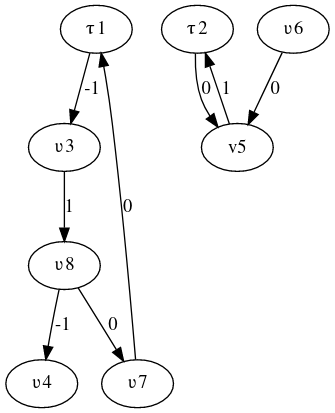
\includegraphics[width=0.3\linewidth]{images/digraph.png}
% Generating the graph requires \usepackage{dot2texi} or \usepackage[pdf]{graphviz}
\iffalse
\begin{dot2tex}[file=cstrnts,scale=0.6]
digraph D {
    t1 [label=<&tau;<SUB>1</SUB>>];
    t2 [label=<&tau;<SUB>2</SUB>>];
    v3 [label=<&upsilon;<SUB>3</SUB>>];
    v4 [label=<&upsilon;<SUB>4</SUB>>];
    v6 [label=<&upsilon;<SUB>6</SUB>>];
    v7 [label=<&upsilon;<SUB>7</SUB>>];
    v8 [label=<&upsilon;<SUB>8</SUB>>];
    v7 -> t1 [label="0"];
    v8 -> v7 [label="0"];
    t2 -> v5 [label="0"];
    v6 -> v5 [label="0"];
    v8 -> v4 [label="-1"];
    v3 -> v8 [label="1"];
    t1 -> v3 [label="-1"];
    v5 -> t2 [label="1"];
}
\end{dot2tex}
\fi
\caption{Example size variable constraints as a weighted directed graph}
\label{fig:digraph}
\end{figure}

%%% Local Variables:
%%% TeX-master: "../main.tex"
%%% TeX-engine: default
%%% End:


\RecCheckLoop then calls $\RecCheck(C, \tau_1, \set{\tau_1, \tau_2}, \upsilon_5)$.
Following its steps, we have:
\begin{enumerate}
    \item $V^\iota = \set{\upsilon_7, \upsilon_8, \upsilon_3}$, and we add the constraints $C' = \tau_1 \sqsubseteq V^\iota$ (subsizing each variable in $V^\iota$).
    \item It is evident that there are no negative-weight cycles in the constraint graph, so $V^- = \emptyset$.
    \item Nothing to be done.
    \item We have $\bigsqcup V^\neq = \set{\upsilon_5, \tau_2}$ and $\bigsqcup V^\iota = \set{\tau_1, \upsilon_3, \upsilon_8, \upsilon_7, \upsilon_4}$.
      Their intersection is empty, so we add no new constraints.
    \item There is no $\infty$ present, so $V^\bot = \emptyset$ and we return the constraints $C \cup C'$.
\end{enumerate}

\RecCheckLoop executes without failure, so \texttt{defBody} indeed has type $\text{Nat}^{\tau_1} \to \text{Nat}^{\tau_2}$.
Erasing this type to a global type for the global definition's type and to a position type for the fixpoint's type, the fully annotated program is then:

\begin{minted}[escapeinside=<>,mathescape=true]{coq}
Def example: Nat<$^\iota$> <$\to$> Nat<$^\iota$> <$\coloneqq$>
  fix<$_{\langle 1 \rangle, 1}$> <$\langle$>f: Nat<$^*$> <$\to$> Nat<$^*$> <$\coloneqq$>
    <$\lambda$>n: Nat. case<$_{\lambda x: \texttt{Nat}. \texttt{Nat}}$> n of
      <$\langle$>O <$\Rightarrow$> O,
       S <$\Rightarrow$> <$\lambda$>n': Nat. f n'<$\rangle \rangle$>.
\end{minted}

\section{Metatheoretical Results}
\label{sec:metatheory}

In this section, we describe the metatheory of \lang.
Some of the metatheory is inherited or essentially similar to past work~\citep{cic-hat-minus,cc-hat-omega,cic-hat},
although we must adapt key proofs to account for differences in subtyping and definitions.
Complete proofs for a language like \lang are too involved to present in full,
so we provide only key lemmas and proof sketches.

In short, \lang satisfies confluence and subject reduction, with the same caveats as in CIC for cofixpoints.
Proofs of strong normalization and logical consistency for \lang remain future work.
% TODO: Why a conjecture and not a proof? Because it hard.
We conjecture how the proofs of strong normalization and consistency should proceed based on past work~\citep{cic-hat-minus,cc-hat-omega,cic-hat}.

\subsection{Confluence}

Recall that we define $\rhd$ as the congruent closure of \reduction and $\rhd^*$ as the reflexive--transitive closure of $\rhd$.

\begin{theorem}[Confluence]
\label{thm:metatheory:confluence}
  If $\gg \vdash e \rhd^* e_1$ and $\gg \vdash e \rhd^* e_2$,
  then there is some term $e'$ such that $\gg \vdash e_1 \rhd^* e'$ and $\gg \vdash e_2 \rhd^* e'$.
\end{theorem}

\begin{proof}[{[sketch]}]
  We use the Takahashi translation technique due to \citet{takahashitrans},
  which is a simplification of the standard parallel reduction technique.
  It uses the Takahashi translation $e^\dagger$ of terms $e$,
  defined as the simultaneous single-step reduction of all
  $\beta\zeta\delta\Delta\iota\mu\nu$-redexes of $e$ in left-most inner-most order.
  The proof is relatively standard thanks to reduction being purely syntactic and untyped.
  % Is it though?
\end{proof}

\subsection{Subject Reduction}
\label{sec:metatheory:sub-red}

Suject reduction does not hold in \lang or in Coq due to the way coinductives are presented.
This is a well-known problem, discussed previously in a sized-types setting by \citet{cc-hat-omega},
on which our presentation of coinductives is based,
as well as by the Coq developers\footnote{The discussion of the problem and suggested solutions can be found here: \url{https://github.com/coq/coq/issues/5288/}.}.

In brief, the current presentation of coinductives requires that cofixpoint reduction be \textit{restricted},
\ie occurring only when it is the target of a case expression.
This allows for strong normalization of cofixpoints in much the same way restricting fixpoint reduction to when the recursive argument is syntactically a fully-applied constructor does.
One way this can break subject reduction is by making the type of a case expression not be convertible before and after the cofixpoint reduction.
As a concrete example, consider the following coinductive definition for conaturals.
\begin{displaymath}
  \seq{\assm{\Conat}{\Type{}}} \coloneqq {\seq{\assm{\Succ}{\Conat \to \Conat}}}
\end{displaymath}
For some motive $P$ and branch $e$, we have the following $\nu$-reduction.
\begin{align*}
  &\caseof*{\erase{P}}{\cofix*{1}{\defn{\omega}{\Conat}{\app{\Succ}{\omega}}}}{\seq{\Succ \Rightarrow e}} \rhd_\nu \\
  &\caseof*{\erase{P}}{\app{\Succ}{(\cofix*{1}{\defn{\omega}{\Conat}{\app{\Succ}{\omega}}})}}{\seq{\Succ \Rightarrow e}}
\end{align*}
Assuming both terms are well-typed, the former has type $\app{P}{(\cofix*{1}{\defn{\omega}{\Conat}{\app{\Succ}{\omega}}})}$ while the latter has type $\app{P}{(\app{\Succ}{(\cofix*{1}{\defn{\omega}{\Conat}{\app{\Succ}{\omega}})}})}$, but for an arbitrary $P$ these are not convertible without allowing cofixpoints to reduce arbitrarily.

\begin{figure}
  \fbox{$\gg \vdash e \reduce_{\beta\zeta\delta\Delta\iota\mu\nu'} e$} \hfill
  \vspace{-3ex}
  \begin{align*}
    \dots & \\
    \gg \vdash q_m & \reduce_{\nu'} \substvec{e_m}{f_k}{q_k} \\
    \textit{where} ~ & \forall i \in \vec{k}, q_i \equiv \cofix{i}{f_k}{t_k}{e_k}
  \end{align*}
  \caption{Reduction rules with unrestricted cofixpoint reduction}
  \label{fig:reduction-alt}
\end{figure}

On the other hand, if we do allow unrestricted $\nu$-reduction as in \autoref{fig:reduction-alt}, subject reduction does hold,
at the expense of normalization,
as a cofixpoint on its own could reduce indefinitely.

\begin{theorem}[Subject Reduction]
  \label{thm:metatheory:sr}
  Let $\Sigma$ be a well-formed signature.
  Suppose that $\nu$-reduction to allows unrestricted reduction of cofixpoints.
  Then $\gg \vdash e : t$ and $e \rhd e'$ implies $\gg \vdash e' : t$.
\end{theorem}

\begin{proof}[{[sketch]}]
  By induction on $\gg \vdash e : t$.  Most cases are straightforward,
  making use of confluence when necessary, such as for a lemma of
  $\Pi$-injectivity to handle $\beta$-reduction in \refrule{app}.
  %
  The case for \refrule{case} where $e \rhd e'$ by $\iota$-reduction relies on the fact that
  if $x$ is the name of a \coinductive type and appears strictly positively in $t$,
  then $x$ appears covariantly in $t$.
  (This is only true without nested \coinductive types, which \lang disallows in well-formed signatures.)

  The case for \refrule{case} and $e$ (guarded) $\nu$-reduces to $e'$ requires an unrestricted $\nu$-reduction.
  After guarded $\nu$-reduction, the target (a cofixpoint) appears in the motive unguarded by a case expression, but must be unfolded to re-establish typing the type $t$.
\end{proof}

\subsubsection{The Problem with Nested Inductives}

\newcommand{\nat}{\const{N}}

Recall from \autoref{sec:typing} that we disallow nested \coinductive types.
This means that when defining a \coinductive type, it cannot recursively appear as the parameter of another type.
For instance, the following definition $\nat$, while equivalent to $\Nat$,
is disallowed due to the appearance of $\nat$ as a parameter of $\Box$.
\begin{align*}
  \seq{\assm{\nat}{\Type{}}} \coloneqq \seq{\assm{\Zero}{\nat}, \assm{\Succ}{\app{\Box}{\nat} \to \nat}}
\end{align*}
Notice that we have the subtyping relation $\nat^\upsilon \leq \nat^{\hat{\upsilon}}$,
but as all parameters are invariant for backward compatibility and need to be convertible,
we do \emph{not} have $\app{\Box^\infty}{\nat^\upsilon} \leq \app{\Box^\infty}{\nat^{\hat{\upsilon}}}$.
But because case expressions on some target $\nat^{\hat{s}}$ force recursive arguments to have size $s$ exactly,
and the target also has type $\nat^{\hat{\hat{s}}}$ by cumulativity,
the argument of $\Succ$ could have both type $\app{\Box^\infty}{\nat^s}$ and $\app{\Box^\infty}{\nat^{\hat{s}}}$, violating convertibility.
We exploit this fact and break subject reduction explicitly with the following counterexample term.
\begin{displaymath}
\begin{array}{l}
  \caseof*{\erase{\abs{\any}{\nat}{\nat^\infty}}}{\app{\Succ}{(\app{\MkBox}{\nat^{\hat{\upsilon}}}{\Zero})}}{\\
  \seq{\Zero \Rightarrow \Zero,\\
  \phantom{\langle} \Succ \Rightarrow \app{(\abs{A}{\Type{}}{\abs{x}{A}{\Zero}})}{(\app{\Box^\infty}{\nat^{\hat{\hat{\upsilon}}}})}}}
\end{array}
\end{displaymath}
By cumulativity, the target can be typed as $\nat^{\hat{\upsilon}^{3}}$ (that is, with size $\hat{\hat{\hat{\upsilon}}}$).
By \refrule{case}, the second branch must then have type $\prod{x}{\app{\Box}{\nat^{\hat{\hat{\upsilon}}}}}{\nat^\infty}$ --- and so it does.
Then the case expression is well typed with type $\nat^\infty$.
However, once we reduce the the case expression, we end up with a term that is no longer well typed.
\begin{displaymath}
  \app{(\abs{A}{\Type{}}{\abs{x}{A}{\Zero}})}
    {(\app{\Box^\infty}{\nat^{\hat{\hat{\upsilon}}}})}
    {(\app{\MkBox}{\nat^{\hat{\upsilon}}}{\Zero})}
\end{displaymath}
By \refrule{app}, the second argument should have type $\app{\Box^\infty}{\nat^{\hat{\hat{\upsilon}}}}$ (or a subtype thereof), but it cannot:
the only type the second argument can have is $\app{\Box^\infty}{\nat^{\hat{\upsilon}}}$.

There are several possible solutions, all threats to backward compatibility.
\CIChat's solution is to require that constructors be fully-applied and that their parameters be bare terms,
so that we are forced to write $\app{\MkBox}{\nat}{\Zero}$.
The problem with this is that Coq treats constructors essentially like functions,
and assuring that they are fully applied with bare parameters would require either reworking how they are represented internally
or adding an intermediate step to elaborate partially-applied constructors into functions whose bodies are fully-applied constructors.
The other solution, as mentioned, is to add polarities back in, so that $\Box$ with positive polarity in its parameter yields the subtyping relation $\app{\Box^\infty}{\nat^{\hat{\upsilon}}} \leq \app{\Box^\infty}{\nat^{\hat{\hat{\upsilon}}}}$.

Interestingly, because the implementation infers all size annotations from a completely bare program,
our counterexample and similar ones exploiting explicit size annotations aren't directly expressible,
and don't appear to be generated by the algorithm, which would solve for the smallest size annotations.
For the counterexample, in the second branch, the size annotation would be (a size constrained to be equal to) $\hat{\upsilon}$.
We conjecture that the terms synthesized by the inference algorithm do indeed satisfy subject reduction even in the presence of nested \coinductives,
although perhaps at the expense of other desired metatheoretical properties,
such as completeness of the algorithm with respect to the typing rules,
which we discuss in the next subsection.

\subsection{Strong Normalization and Logical Consistency}\label{sec:metatheory:sn}

In ongoing work%
\footnote{To be submitted as an undergraduate thesis by Yufeng Li
  under the supervision of Bruno Barras.}  on a variant of \lang
called \langAnother, strong normalization has been proven with a
set-theoretic model construction equipped with realisability
candidates based on \citet{barras-thesis}.
%
From challenges encountered during the strong normalization proof, we
learnt that in order to build a set-theoretic model for normalization,
formulation of sized types in CIC has to satisfy additional
requirements.
%
This section explains what these additional requirements are by
motivating each of them from necessities that arose out of the proof
attempt.

At a high level, the proof uses a semantics-first set-theoretic model
construction equipped with realisability candidates based on the works
of \citet{barras-thesis}.
%
To simplify the presentation, \langAnother does not deal with the sort
$\Set$, mutual fixpoints, cofixpoints, local definitions, or global
declarations; for the proof to work, \langAnother requires additional
nontrivial changes relative to \lang:
%
\begin{itemize}
  %
  \item Fixpoint type annotations require explicit size annotations
  (\ie are no longer merely position terms), explicitly abstract over
  a size variable, and are explicitly applied to a size expression:
  %
  \begin{align*}
    \left\{\kw{fix}^\upsilon ~ f : \prod{n}{\Nat^\upsilon}{u} \coloneqq e\right\}_s
    \tag{$\star$}\label{eqn:new-fix}
  \end{align*}
  %
  Here, $f$ is said to \emph{bind} the size variable $\upsilon$ in $e$
  and the subscript size expression $s$ states that one may only call
  the fixpoint recursor on inputs of size $s$ or less.
  %
  In correspondence, the typing rule no longer erases the type, and
  the size in the fixpoint type is fixed:
  %
  \begin{mathparpagebreakable}
    \inferrule*[right=\defrule{fix-another}]
    { \Gamma (f : \prod{n}{\Nat^\upsilon}{u}) \vdash e :
      \prod{n}{\Nat^{\hat{\upsilon}}}{\subst{u}{\upsilon}{\hat{\upsilon}}} }
    { \Gamma \vdash \left\{\kw{fix}^\upsilon ~ f : \prod{n}{\Nat^\upsilon}{u}\right\}_s \coloneqq e :
      \prod{n}{\Nat^{s}}{\subst{u}{\upsilon}{s}} }
  \end{mathparpagebreakable}
  %
  \item Rather than inductive definitions in general, only predicative
  W-types are considered.
  %
  W-types can be defined as an inductive type:
  %
  \begin{mathparpagebreakable}
    \seq{\app{\W}{(\assm{A}{U})}{(\assm{B}{A \rightarrow U})}} \coloneqq
    \seq{\assm{\Sup}{(\assm{a}{A}) \rightarrow (\assm{f}{\app{B}{a} \rightarrow \app{\W}{A}{B}})
        \rightarrow \app{\W}{A}{B}}}
  \end{mathparpagebreakable}
  %
  Predicative W-types only allow $U$ to be $\Type{i}$ (or $\Set$, but
  \langAnother does not deal with $\Set$), while impredicative W types
  also allow it to be $\Prop$.
  %
  Including impredicative W types as well poses several technical
  challenges to the realisability semantics.
  %
  % Inductive types are replaced by predicative W-types in order
  % to alleviate some syntactic burden of dealing with strict positivity
  % conditions.
  % %
  % However, \citet{w-types,polynomial-functors-w,barras-thesis} have
  % shown that W-types are powerful enough to encode many strictly
  % positive inductive definitions, including nested inductive types and
  % inductive types with non-uniform parameters.
  % %
  % Including impredicative inductive types to the strong normalization
  % model, on the other hand, does pose several technical challenges
  % related to the realisability semantics.
  %
  \item As it is the case for most set-theoretic model constructions,
  reduction, subtyping, and conversion are typed.
  %
  That is, each judgement requires the type of the terms,
  and the derivation rules may have as typing judgements as premises.
  %
\end{itemize}

As a consequence of treating fixpoint recursors as binders for size
variables as in \eqref{eqn:new-fix}, when we reduce a fixpoint
recursor, we need to replace the corresponding bound size variable in
its body.
%
Work under some context $\Gamma$ and take the following fixpoint
recursor as running example:
%
\begin{align*}
  F \triangleq \left\{\kw{fix}^\upsilon ~ f : \Nat^\upsilon \to \Nat^\upsilon \coloneqq e\right\}_{\hat{s}}
  \label{eqn:fix-example}\tag{$\varheartsuit$}
\end{align*}
%
Let $t$ be some $\Nat$ in constructor form (\ie $t = \Succ ~ n$ or
$t = \Zero$) where $t$ has size $\hat{s}$.
%
Then, as fixpoint recursors bind size variables, when we apply $F$ to
$t$, we specialise $\upsilon$ to $\hat{s}$, so $\mu$-reduction should
say
%
\begin{align*}
  \app{F}{t} \rhd \app{\subst{\subst{e}{\upsilon}{s}}{f}{
  \left\{\kw{fix}^\upsilon ~ f : \Nat^\upsilon \to \Nat^\upsilon \coloneqq e\right\}_{s}
  }}{t}
  \label{eqn:mu-example}\tag{$\vardiamondsuit$}
\end{align*}
%
In particular, note that we substitute $s$ instead of $\hat{s}$ for
$\upsilon$ and we substitute for $f$ not $F$ but the fixpoint recursor
specialized to stage $s$.
%
This corresponds to the sized typing rule for fixpoint recursors:
$\left\{\kw{fix}^\upsilon ~ f : \Nat^\upsilon \to \Nat^\upsilon
  \coloneqq e\right\}_{s}$ is a function taking inputs of size $s$, so
on input $t$ of size $\hat{s}$, the body $e$ can recursively call
itself, but only on inputs of size $s$.

Because these changes violate backward compatibility, they cannot be adopted in \lang.
%
The current literature suggests that \langAnother and \lang may be
proven to be equivalent such that strong normalization (and therefore
logical consistency) of \langAnother implies that they hold in \lang.
More specifically, \cite{conversion} show that a typed and an untyped
convertibility in a Martin--L\"of type theory (MLTT) imply each other;
and \citet{w-types, polynomial-functors-w} show that W types in an
extensional MLTT can encode well-formed inductive types, including
nested inductive types (while \citet{hofmann} shows that extensional
MLTT is a conservative extension of intensional MLTT).
%
But even with a modified version of \lang, proving strong
normalization was still not easy.
%
The explanation is given as follows:
%
\begin{itemize}
  %
  \item The intuition that sized types ensure termination seems to be
  difficult to formalize in a set-theoretic model without further
  restrictions on the type-checking rule for fixpoint recursors.
  %
  This restriction is called size irrelevance and is explained in
  \Cref{sec:size-irrel}.
  %
  \item In the expected sizes-as-ordinals interpretation, finding an
  ordinal corresponding to the $\infty$ size in a given term seems to
  be a task more involved than expected.
  %
  Such an ordinal interpretation of $\infty$ is significant to showing
  $\mu$-reduction is set-theoretically sound, and is explained in
  \Cref{sec:infty-compute}.
  %
\end{itemize}

\subsubsection{Size Irrelevance}\label{sec:size-irrel}
%
The sized typing rule for fixpoint recursors appears particularly
syntactically appealing and is supposed to ensure termination.
%
Intuitively, the key to why sized types ensure termination is because
recursion happens on smaller elements.
%
Take the situation of \eqref{eqn:fix-example} as example.
%
Whenever the body $e$ recursively calls $f$, since we know that the
recursive call happens on strictly smaller elements, if we replace
instances of $f$ in the body $e$ with two functions $\varphi,\varphi'$
that behave identically on smaller elements then $e$ should not be
able to tell apart $\varphi,\varphi'$.
%
In order to construct a strong-normalization model in set theory, one
would like to formalise this idea of $e$ not being able to tell apart
functions that agree on smaller values.
%
This section tries to show why doing so is perhaps not completely
straightforward.

In the strong normalization model, we interpret terms and types as
their natural set-theoretic counterparts and size variables as
ordinals.
%
For $\rho$ a valuation of $\Gamma$ mapping variables to sets and $\pi$
mapping size variables to ordinals, denote by $\Val(M)_\rho^\pi$ the
set-theoretic denotation of the term $M$ under these valuations.
%
Now, suppose $s=\infty$ and consider how one would define
$\Val(F)_\rho^\pi$.
%
Since $s=\infty$, intuitively, $F$ should be the fixpoint of $e$.
%
So, we take some initial approximation of the fixpoint of the value of
$e$ and at every stage, improve the approximation by evaluating $e$ on
the prior approximation, until the approximation cannot be further
improved, which means we have reached a fixpoint of the iteration.

For the sake of simplicity, assume that for all ordinals $\alpha$, the
value of $\Nat^\upsilon$ where $\upsilon$ is interpreted as $\alpha$
is just
$\Val(\Nat^\upsilon)_\rho^{\subst{\pi}{\upsilon}{\alpha}} =
\McN^\alpha$ where $(\McN^\alpha)_\alpha$ is an $\subseteq$-increasing
family sets constant beyond $\omega$.
%
Putting $D_0$ to be some well-chosen singleton set and
$D_\alpha \triangleq \Val(\Nat^\upsilon \to
\Nat^\upsilon)_\rho^{\subst{\pi}{\upsilon}{\alpha}} = \McN^\alpha \to
\McN^\alpha$, the usual approach is to iterate up until the least
fixpoint of the operator
%
\begin{align*}
  \varphi \triangleq
  (\alpha \in \Ord) \mapsto (\psi \in D_\alpha) \mapsto \Val(e)_{\subst{\rho}{f}{\psi}}^{\subst{\pi}{\upsilon}{\alpha}}
  \tag{$e$-iter}\label{eqn:e-iter}
\end{align*}
%
starting from the initial approximation $\varphi_0 \in D_0$ and
setting the $(\alpha+1)$-th approximation $\varphi_{\alpha+1}$ as
$\varphi(\varphi_\alpha)$.
%
The typing rule for $F$ given by \refrule{fix-another} is sufficient
to ensure that each $\varphi_\alpha \in D_\alpha$.
%
However, this alone is not enough: we want the sequence
$(\varphi_\alpha)_\alpha$ to be convergent.

What would be a sufficient condition for convergence?
%
Note that $(\varphi_\alpha)_\alpha$ is obtained by successively
improving upon approximations of the fixpoint of $\varphi$, so one
would expect that
%
\begin{align*}
  \varphi_\alpha(x) = \varphi_\beta(x) \text{ for all } x \in \McN^\alpha \subseteq \McN^\beta
  \label{eqn:size-irrel}\tag{\textsc{size-irrel}}
\end{align*}
%
This expresses a condition of size irrelevance: size variables bound
by fixpoint recursors can only be used to restrict their domains, and
should not be used to affect the value of computation.
%
And it turns out that \eqref{eqn:size-irrel} is enough to ensure
$(\varphi_\alpha)_\alpha$ converges to $\varphi_\omega$.
%
So, it remains to prove \eqref{eqn:size-irrel}.
%
Assume inductively it holds $\alpha,\beta$ and we would like to prove
it for $\alpha+1,\beta+1$, so that the goal is to show, for
$x \in \McN^{\alpha+1} \subseteq \McN^{\beta+1}$,
%
\begin{align*}
  \Val(e)_{\subst{\rho}{f}{\varphi_\alpha}}^{\subst{\pi}{\upsilon}{\alpha}}(x) =
  \Val(e)_{\subst{\rho}{f}{\varphi_\beta}}^{\subst{\pi}{\upsilon}{\beta}}(x)
\end{align*}
%
By the intuitive understanding of sized typing, on input
$x \in \McN^{\alpha+1}$ of size $\alpha+1$, the body $e$ can only
recursively call $f$ on inputs of size at most $\alpha$.
%
And inductively, $\varphi_\alpha$ behaves identically to
$\varphi_\beta$ on inputs of size at most $\alpha$.
%
So, $e$ on input $x \in \McN^{\alpha+1}$ should not be able to
distinguish between $\varphi_\alpha$ and $\varphi_\beta$, thus
ensuring the above equality.
%
However, just from \refrule{fix-another}, it seems that one cannot
easily conclude that $e$ cannot tell apart $\varphi_\alpha$ and
$\varphi_\beta$.

This problem was encountered also by \citet{barras-thesis}, who solved
it by introducing a special typing mode called size irrelevance typing
and marker for the $\Pi$-types of fixpoint recursors.
%
We have used a similar solution to get around this problem in the
strong normalization proof of the alternative formulation of \lang.
%
However, in the size irrelevance typing of \citet{barras-thesis},
there was the requirement that fixpoint recursors can never occur as
arguments to other functions in their defining body.
%
For example, in order for $e$ to pass size irrelevance typing, $e$
cannot contain a sub-expression of the form $(\app{M}{f})$.
%
\todo{
  %
  (The main idea I want to express is basically that we type the
  bodies of fixpoint recursors in this size irrelevance mode.
  %
  And size
  irrelevance is supposed to put on more restrictions in addition to
  the existing sized typing rules.
  %
  So it seems natural to ask how restrictive is size irrelevance
  typing compared to usual sized typing.
  %
  And it turns out that size irrelevance typing is not restrictive by
  that much.)
  %
}
%
We were able to get rid of this requirement in the strong
normalization proof of this alternative formulation of \lang.
%
In fact, the typing rules allowed for size irrelevance typing can be
expanded to include counterparts for almost all of the ``normal''
typing rules.

An alternative approach seems uses a model involving PERs, where the
PERs are designed to ensure size irrelevance.
%
In any case, it seems that an inherent restriction of size irrelevance
is one may not have a recursive function $F$ with behaviours such as
$\app{F}{n} \approx \Nat^\upsilon \to ...n\text{ times}... \to
\Nat^\upsilon$ or even $\app{F}{n} \approx \Nat^\upsilon$ where
$\upsilon$ is the size variable bound by $F$.
%
\citet{cic-hat-minus} has a similar restriction present in
\CIChatminus, and this restriction matches the intuition of
size irrelevance.
%
If $\app{F}{n} \approx \Nat^\upsilon$ then the value of $F$ on an
input $n$ depends on the size $\upsilon$, which precisely the
behaviour size irrelevance aims to forbid.
%
On the other hand, $\app{F}{n} \approx \Nat^\infty \to
...n\text{ times}...\to\Nat^\infty$ does adhere to size irrelevance.

\subsubsection{Computation of $\infty$}\label{sec:infty-compute}
%
A second challenge in constructing the set-theoretic model is the
problem of justifying $\mu$-reduction set-theoretically.
%
Due to the sizes-as-ordinal interpretation of sizes, this problem
seems to be related to the ordinal interpretation of the $\infty$
size.

Take the $\mu$-reduction equation in \eqref{eqn:mu-example} as an
example.
%
Once again, assume $s=\infty$ and \eqref{eqn:size-irrel} holds, so that
$(\varphi_\alpha)_\alpha$ is constant beyond $\omega$.
%
Then, by the previous discussion, the value of $F$ and of
$\left\{\kw{fix}^\upsilon ~ f : \Nat^\upsilon \to \Nat^\upsilon
  \coloneqq e\right\}_{s}$ are both taken to be
$\varphi_\omega = \varphi_{\kappa}$ for all $\kappa \geq \omega$.
%
Then, by substitutivity, the $\mu$-reduction equation in
\eqref{eqn:mu-example} should say, for sufficiently large
$\kappa \geq \omega$,
%
\begin{align*}
  \Val(\app{F}{t})_\rho^\pi =
  \Val(\app{\subst{\subst{e}{\upsilon}{\infty}}{f}{
  \left\{\kw{fix}^\upsilon ~ f : \Nat^\upsilon \to \Nat^\upsilon \coloneqq e\right\}_{\infty}
  }}{t})_\rho^\pi
\end{align*}
%
By substitutivity and the fact that $(\varphi_\alpha)_\alpha$ is
constant beyond $\kappa$, this is equivalent to showing that
%
\begin{align*}
  \varphi_{\kappa+1}(\Val(t)_\rho^\pi) =
  \Val(\subst{e}{\upsilon}{\infty})_{\subst{\rho}{f}{\varphi_\kappa}}^{\pi}(\Val(t)_\rho^\pi)
\end{align*}
%
But
$\varphi_{\kappa+1} =
\Val(e)_{\subst{\rho}{f}{\varphi_\kappa}}^{\subst{\pi}{\upsilon}{\kappa}}$,
to show the above equality, it remains to move the
$\subst{e}{\nu}{\infty}$ in the syntax into the valuation
$\subst{\pi}{\nu}{\kappa}$, for some large $\kappa$.

More generally, it seems true that for all terms $M$ and valuations
$\rho$ and $\pi$, and size variables $\nu$, there is some ordinal
$\Infty(M;\nu)_\rho^\pi$ with the $\infty$-substitutivity property:
%
\begin{align*}
  \kappa \geq \Infty(M;\nu)_\rho^\pi \text{ implies }
  \Val(\subst{M}{\nu}{\infty})_\rho^\pi = \Val(M)_\rho^{\subst{\pi}{\nu}{\kappa}}
  \label{eqn:infty-subst}\tag{$\infty$-subst}
\end{align*}
%
This equality somehow expresses the idea that $\Infty(M;\nu)_\rho^\pi$
closes off all inductive types annotated with $\nu$ in $M$, so
$\Infty(M;\nu)_\rho^\pi$ is the denotation of $\infty$ for $\nu$ in
$M$ under $\rho$ and $\pi$.
%
Intuitively, we know this ordinal $\Infty(M;\nu)_\rho^\pi$ exists,
because the strict positivity condition ensures that by iterating the
operator associated with an inductive type up to its closure ordinal,
we eventually reach their fixpoints.
%
Since there can only be finitely many inductive types in $M$, an
ordinal with the $\infty$-substitutivity property is just the
supremum of these closure ordinals.

However, the computation of $\Infty(M;\nu)_\rho^\pi$ is complicated by
the fact that in $M$, the size variable $\nu$ can be annotated to more
than one inductive type.
%
For example, in $M$, the size variable $\nu$ can be annotated to both
$\Nat^\nu$ and $I^\nu$, where $I$ is some inductive type with a
different closure ordinal than $\Nat$.
%
In fact, it turned out that computing $\Infty(M;\nu)_\rho^\pi$ was
much more involved than initially expected.

\subsubsection{Relation to \lang and Coq}
%
Let us conclude this section by recalling that Coq itself is not
strongly normalizing, only weakly normalizing.
%
\footnote{At least, the
  underlying calculus is not. The counterexample ``normalizes'' to a
  stack overflow on machine with finite memory.}

\begin{minted}{coq}
Definition cbv_omega := fix f (n : nat) := let x := f n in O.
\end{minted}

This is a side-effect of relaxing the guard condition to enable more
sound programs to type check.
%
Ideally, sufficiently expressive sized typing will allow us to replace
the guard condition entirely and regain strong normalization in Coq.

However, an intermediate goal may be to achieve only weak
normalization of \lang.
%
This would also maintain backward compatibility with Coq, although it
is unclear if counterexamples like the above are ever desired in user
programs.

%%% Local Variables:
%%% TeX-master: "../main.tex"
%%% TeX-engine: default
%%% End:

\section{Related Work}\label{sec:related}

The history of sized types is vast and varied.
Extensive prior accounts are given in dissertations by \citet{lambda-hat-diss} and \citet{abel-diss}.
Here, we focus on two lineages towards sized dependent type theories: first, the more-or-less direct ancestry of \lang, and second, a contrasting line of work on type systems with explicit higher-order sized types.

\subsection{Ancestry of \titlelang}

Perhaps the most well-known work on sized types is by \citet{hughes},
who introduce sized types for a Hindley--Milner type system with \coinductives and a size inference algorithm,
as well as the term ``sized types''.
Their size algebra is more expressive than ours, with size addition $s_1 + s_2$ and constant multiplication $n \times s$.
Independently, \citet{ccr} introduces \CCR, a Calculus of Constructions (CoC) with \textit{guarded types},
a type-based termination checking alternative to the earlier syntactic guard condition~\citep{guard-condition}.
There, types are guarded with a type operator $\widehat{\ph}$,
similar to the later modality $\rhd \ph$ in modern guarded type theories.
Based on a semantic interpretation of \CCR,
\citet{acg} introduce a simply-typed lambda calculus (STLC) with coinductives with \textit{type labels},
corresponding roughly to size annotations with successor sizes.

Following this, \citet{lambda-hat} and \citet{lambda-hat-diss} introduce \lambdahat,
another STLC with inductives and size annotations with the same size algebra we use,
although they are instead called \textit{stages}.
It improves upon the work of \citet{acg} by adding an implicit form of size polymorphism:
the position size variable of fixpoint types are substituted by an arbitrary size expression,
just as in \refrule{fix}.
\citet{f-hat} extend \lambdahat to System F with \Fhat, and introduce and prove correct a size inference algorithm.
This includes the \RecCheck algorithm that we use.
They continue on to extend \Fhat with \textit{sized products} (that is, pairs with size annotations) in \FXhat~\citep{fx-hat}, whose size expressions include size addition, and to CIC in \CIChat~\citep{cic-hat}.
Our size inference algorithm is based directly on that of \CIChat.
We add to it global and local definitions and explicitly treat mutually-defined \coinductives and \cofixpoints,
while removing polarities and subtyping based on these polarities.

However, normalization of \CIChat is only a conjecture; it is later proven for the restricted language \CIChatminus by \citet{cic-hat-minus-nat} (with only naturals) and by \citet{cic-hat-minus} (with inductive types).
The restrictions include disallowing size variables in the bodies of functions, in the arguments of applications, in the branches of case expressions, and in the indices of inductives; erasing the parameters to constructors; and disallowing strong elimination to types with size variables.
We remove these restrictions to allow using sized definitions and for backward compatibility with Coq.

Our typing rules and inference algorithm for coinductives and cofixpoints are based on \CChatomega~\citep{cc-hat-omega},
which extends CoC with sized coinductive streams.
Further extensions to the size algebra are linear sized types in \CIChatl~\citep{cic-hat-l},
which adds constant multiplication to a sized CoC with naturals and streams;
and well-founded sized types in \CIChatsub~\citep{wellfounded},
which changes the premise type checking the \cofixpoint body in Rules \refnorule{fix} and \refnorule{cofix}
to the recursive reference having \emph{any} smaller size according to the subsizing rules,
rather than the direct predecessor.
All three include size inference algorithms similar to that of \CIChat.

There are prototype implementations of \CIChatminus~\citep{cicminus} and \CIChatsub~\citep{cic-wf}.
It appears that there were also plans to implement sized types in Coq by \citet{coq-hat}, but seem to be abandoned.

\subsection{Higher-Order Sized Types}

For the purposes of size inferrability from unannotated code,
the type systems from \lambdahat up to \CIChat and its variations treat sizes as merely annotations
and feature only what can be considered as prenex size polymorphism.
On the other hand, \citet{abel-diss} introduces \Fomegahat, a sized type system for System F$_\omega$ that treats size as a kind,
which therefore allows for higher-order size polymorphism via explicit quantification.
While \Fomegahat subsumes \Fhat and uses the same size algebra,
it uses recursive and corecursive type constructors ($\mu$- and $\nu$-types) rather than inductive (and coinductive) type definitions.

Higher-order sized types of the same flavour are implemented in a dependently-typed setting in MiniAgda~\citep{miniagda}.
To avoid inconsistencies introduced by the interplay between sized types and pattern matching,
it also introduces bounded size patterns $\upsilon_1 < \upsilon_2$.
\citet{flationary} expands upon the theoretical side with bounded size quantification $\forall \upsilon \mathrel{<} s\mathpunct{.} t$ and well-founded recursion on sizes,
which are also implemented in MiniAgda.
\citet{f-omega-cop} combine well-founded sized types and copatterns for System F$_\omega$ with \corecursive type constructors in \Fomegacop (which was cited as the inspiration for \CIChatsub).

\cite{nbe} prove normalization of a higher-order sized dependent type theory with naturals, but without bounded size quantification.
To our knowledge, this is the only formalization of higher-order sized dependent types in the literature.

Sized types with higher-order bounded size quantification are implemented in Agda\footnote{For Agda's documentation on sized types, see \url{https://agda.readthedocs.io/en/latest/language/sized-types.html}.};
however, it is known to be inconsistent\footnote{For a detailed discussion on the issue, see \url{https://github.com/agda/agda/issues/2820}.}.
In short, it is possible to express the well-foundedness of sizes within Agda,
but the infinite size $\infty$ itself is \emph{not} well-founded,
as $\infty + 1 = \infty$ and $\infty < \infty$ hold,
making it possible to derive a contradiction.

%%% Local Variables:
%%% TeX-master: "../main.tex"
%%% TeX-engine: default
%%% End:

\section{Perspectives and the Future of Sized Types}
\label{sec:conclusion}

We have introduced \lang, a sized type system based on CIC and made to be compatible with Coq,
more than a decade since (prenex, fully-inferrable) sized types for CIC were first introduced in \CIChat and \CIChatminus.
And yet, despite good metatheoretical properties having been established for \CIChatminus,
no functioning attempt at implementing sized types in Coq has previously been made.
This we have done, finding significant performance problems caused by size inference for definitions yielding an explosion in size variables.

This doesn't necessarily spell doom for \lang.
The seasoned type system implementor may employ implementational tricks to improve performance in practice.
Perhaps with some program analysis of how definitions are used, certain size variables known to be irrelevant could immediately be instantiated to the infinite size;
maybe a dependency analysis would reveal which definitions need to be checked with the sized typing flag turned on.
Our na\"ive implementation tries to be as general as possible to accept as many programs as possible,
and heuristics could be used to guess where and why the user wants to use sized types,
whittling down the number of open possibilities for size-inferred programs.

But all of these feel like arbitrary and potentially fragile hacks---and perhaps it's because they \emph{are}.
We have discussed some more sensible solutions to not only the performance problems but also the theoretical ones:
Why don't we explicitly quantify over the size variables of a definition to specify which ones are actually relevant?
Why don't we require that all recursive arguments be marked?
Why not solve the problem of nested inductives using polarities?
but we immediately shoot them down because they require additional work from the user's perspective and therefore violate the philosophy of backward compatibility.
Perhaps this philosophy maintained for more than a decade of past work from \lambdahat to \CIChatsub is \emph{wrong}.

So far, size inference seems to work for programs because the notion of programs were merely single terms.
Inference was merely extracting hidden information already present in the term.
The moment we introduce a little modularity with definitions,
we don't have concrete information on how these definitions will be used,
and by being as general as possible to accommodate all usages,
we end up with terrible performance.
Inference becomes a guessing game we are losing.

If we make size quantification, abstraction, and application explicit,
then there won't be any more size variables involved than are strictly necessary.
To ease the tedious burden of all the extra annotations from the user,
sizes that can be deduced could be marked as implicit and filled in by the elaborator, as is done for terms.
In contrast to inference, elaboration merely deduces information already available,
and fails as soon as more information is required,
rather than trying to heuristically fill in the gaps itself.
Another benefit of explicit sized types is that it can easily be extended to higher-order size quantification.
This appears to be the best future direction for sized types;
after all, Agda is still to date the only practical proof assistant with sized types.

So is sized typing for Coq practical?
Our answer is that it might be---but only if we allow ourselves to ask users to put in a little work as well.

%%% Local Variables:
%%% TeX-master: "../main.tex"
%%% TeX-engine: default
%%% End:


\paragraph*{Conflicts of Interest.} None.

\bibliographystyle{JFPlike}
\bibliography{main.bib}

\clearpage
\appendix

\section{Reduction, Convertibility, Takahashi Translation}\label{sec:red-conv-trans}

\begin{figure}
\begin{flushleft}
\fbox{$\gg \vdash T \reduce_{\beta\zeta\delta\Delta\iota\mu\nu} T$}
\end{flushleft}

\vspace{-3ex}

\begin{mathpar}
  \inferrule*[right=\defnamerule{beta}{$\beta$}]{~}
    {\gg \vdash \app{(\abs{x}{t^\circ}{e_1})}{e_2} \reduce_\beta \subst{e_1}{x}{e_2}}
  \and
  \inferrule*[right=\defnamerule{zeta}{$\zeta$}]{~}
    {\gg \vdash \letin{x}{t^\circ}{e_1}{e_2} \reduce_\zeta \subst{e_2}{x}{e_1}}
  \and
  \inferrule[\defnamerule{delta-local}{$\delta$-local}]
    {(x : t \coloneqq e) \in \Gamma \and \SV(e, t) = \vec{\upsilon_i}}
    {\gg \vdash x^{\seq{s_i}} \reduce_\delta e \overline{[\upsilon_i \coloneqq s_i]}}
  \and
  \inferrule[\defnamerule{Delta-global}{$\Delta$-global}]
    {(\Defn{x}{t}{e}) \in \Gamma_G \and \SV(e, t) = \vec{\upsilon_i}}
    {\gg \vdash x^{\seq{s_i}} \reduce_\Delta e \overline{[\upsilon_i \coloneqq s_i]}}
  \and
  \inferrule*[right=\defnamerule{iota}{$\iota$}]{~}
    {\gg \vdash \caseof{P^\circ}{(\app{c_\ell}{\vec{p}}{\vec{a}})}{c_j}{e_j} \reduce_\iota \app{e_\ell}{\vec{a}}}
  \and
  \inferrule*[right=\defnamerule{mu}{$\mu$}]
    {q_i = \fix{\seq{n_k}, i}{f_k}{t_k}{e_k} \and \norm{\vec{b}} = n_m - 1}
    {\gg \vdash \app{q_m}{\vec{b}}{(\app{c_\ell}{\vec{p}}{\vec{a}})}
      \reduce_\mu \app{\substvec{e_m}{f_k}{q_k}}{\vec{b}}{(\app{c_\ell}{\vec{p}}{\vec{a}})}}
  \and
  \inferrule*[right=\defnamerule{nu}{$\nu$}]
    {q_i = \cofix{i}{f_k}{t_k}{e_k}}
    {\gg \vdash \caseof{P^\circ}{(\app{q_m}{\vec{b}})}{c_j}{a_j}
      \reduce_\nu \caseof{P^\circ}{(\app{\substvec{e_m}{f_k}{q_k}}{\vec{b}})}{c_j}{a_j}}
\end{mathpar}
\caption{Reduction rules}
\label{fig:reduction-full}
\end{figure}

\begin{figure}
\begin{flushleft}
\fbox{$\gg \vdash T \reduce_{\beta\zeta\delta\Delta\iota\mu\nu'} T$}
\end{flushleft}

\vspace{-6ex}

\begin{mathpar}
  \vdots
  \\
  \inferrule*[right=\defnamerule{nupr}{$\nu'$}]
    {q_i = \cofix{i}{f_k}{t_k}{e_k}}
    {\gg \vdash q_m
      \reduce_{\nu'} \substvec{e_m}{f_k}{q_k}}
\end{mathpar}
\caption{Reduction rules (with unrestricted cofixpoint reduction)}
\label{fig:reduction-full-unrestricted}
\end{figure}

\begin{figure}
\begin{flushleft}
\fbox{$\gg \vdash T \conv T$}
\end{flushleft}

\vspace{-3ex}

\begin{mathpar}
  \inferrule[\defnamerule{conv-red}{conv-$\reduce^*$}]
    {\gg \vdash e_1 \reduce^* e \\\\
      \gg \vdash e_2 \reduce^* e}
    {\gg \vdash e_1 \conv e_2}
  \and
  \inferrule[\defnamerule{conv-eta-r}{conv-$\eta$-l}]
    {\gg \vdash e_1 \reduce^* \abs{x}{\erase{t}}{e} \\\\
      \gg \vdash e_2 \reduce^* e'_2 \\\\
      \gg (x:t) \vdash e \conv e'_2 ~ x}
    {\gg \vdash e_1 \conv e_2}
  \and
  \inferrule[\defnamerule{conv-eta-1}{conv-$\eta$-r}]
    {\gg \vdash e_1 \reduce^* e'_1 \\\\
      \gg \vdash e_2 \reduce^* \abs{x}{\erase{t}}{e} \\\\
      \gg (x:t) \vdash e'_1 ~ x \conv e}
    {\gg \vdash e_1 \conv e_2}
\end{mathpar}
\caption{Convertibility rules}
\label{fig:conversion}
\end{figure}


\autoref{fig:reduction-full} lists the complete definitions for all reduction rules, including our new rules for $\delta$- and $\Delta$-reduction.
Notice that in fixpoints, the $n_m$th recursive argument needs to be an applied constructor, while cofixpoints can only be reduced as a case expression target.
These conditions are required for strong normalization.
However, this restricted cofixpoint unfolding causes issues with subject reduction~\cite{cc-hat-omega}.
\autoref{fig:reduction-full-unrestricted} presents an alternate unrestricted nonterminating $\nu'$-reduction of cofixpoints outside of case expressions so that subject reduction holds at the cost of normalization.

We define $\reduce$ as the least compatible closure of $\reduce_{\beta\zeta\delta\Delta\iota\mu\nu}$, $\reduce_n$ as the $n$-step reduction of $\reduce$, and $\reduce^*$ as the reflexive--transitive closure of $\reduce$.
Convertibility ($\approx$) is the symmetric closure of $\reduce^*$ up to $\eta$-expansion, and is formally defined in \autoref{fig:conversion}.

The Takahashi translation $e^\dagger$ of a term $e$~\cite{takahashitrans} is used in our proof of confluence.
Informally, we define it as the simultaneous single-step reduction of all $\beta\zeta\delta\Delta\iota\mu\nu$-redexes of $e$ in left-most inner-most order.
We further define $e^{n\dagger}$ as the $n$-step Takahashi translation of $e$.

\section{Well-Formedness of (Co)Inductive Definitions}\label{sec:wf-ind}

In this section we define what it means for a \coinductive definition to be \emph{well-formed}, including some required auxilliary definitions.
A signature is then well-formed if each of its \coinductive definitions are well-formed.
Note that although we prove subject reduction for \lang without nested inductive types, we include their definitions for completeness.

\begin{definition}[Strict Positivity]
  Given some existing sigature $\Sigma$, the variable $x$ occurs \emph{strictly positively} in the term $t$, written $x \POS t$, if any of the following holds:

  \begin{itemize}
    \item $x \notin \FV(t)$
    \item $t \conv x ~ \vec{e}$ and $x \notin \FV(\vec{e})$
    \item $t \conv \prod{x}{u}{v}$ and $x \notin \FV(u)$ and $x \POS v$
  \end{itemize}

  If nested inductive types are permitted, then $x \POS t$ may hold if the following also holds:

  \begin{itemize}
    \item $t \conv I_k^\infty ~ \vec{p} ~ \vec{a}$ where
      $\langle \Delta_p \vdash I_i ~ \_ : \_ \rangle \coloneqq \langle c_j : \prodctx{\Delta_j}{I_j ~ \dom{\Delta_p} ~ \vec{t}_j} \rangle \in \Sigma$
      for some $k \in \vec{\imath}$ and all of the following hold:
      \begin{itemize}
        \item $\norm{\vec{p}} = \norm{\Delta_p}$
        \item $x \notin \FV(\vec{a})$
        \item For every $j$, if $I_j = I_k$, then $x \nPOS_{I_k} \subst{(\prodctx{\Delta_j}{I_j ~ \vec{p} ~ \vec{t}_j})}{\dom{\Delta_p}}{\vec{p}}$
      \end{itemize}
  \end{itemize}
\end{definition}

\begin{definition}[Nested Positivity]
  Given some existing signature $\Sigma$, the variable $x$ is \emph{nested positive} in $t$ of $I_k$, written $x \nPOS_{I_k} t$, if
  $\langle \Delta_p \vdash I_i ~ \_ : \_ \rangle \coloneqq \_ \in \Sigma$ for some $k \in \vec{\imath}$
  and any of the following holds:

  \begin{itemize}
    \item $t \conv I_k^\infty ~ \vec{p} ~ \vec{a}$ and $\norm{\vec{p}} = \norm{\Delta_p}$ and $x \notin \FV(\vec{a})$
    \item $t \conv \prod{x}{u}{v}$ and $x \POS u$ and $x \nPOS_{I_k} v$
  \end{itemize}

  In short, $x \nPOS_I t$ if $t \conv \prodctx{\Delta}{I ~ \vec{p} ~ \vec{a}}$ and $x \POS \Delta$ and $x \notin \FV(\vec{a})$.
\end{definition}

\begin{definition}[Constructor Type]
  The term $t$ is a constructor type for $I$ when:

  \begin{itemize}
    \item $t = I ~ \vec{e}$; or
    \item $t = \prod{x}{u}{v}$ where $x \notin \FV{u}$ and $v$ is a constructor type for $I$; or
    \item $t = u \to v$ where $x \POS u$ and $v$ is a constructor type for $I$.
  \end{itemize}

  Note that in particular, this means that $t = \prodctx{\Delta}{I ~ \vec{e}}$ such that $I \POS u$
  for every $u \in \codom{\Delta}$, and the recursive arguments of $t$ are not dependent.
\end{definition}

\begin{definition}[Well-formedness of \Coinductive Definitions]
  Suppose we have some signature $\Sigma$ and some global environment $\Gamma_G$. Consider the following \coinductive definition, where $\vec{p} = \dom{\Delta_p}$.
  $$\Delta_p \vdash \langle I_i ~ \vec{p} : \prodctx{\Delta_i}{\varw_i} \rangle \coloneqq \langle c_j : \prodctx{\Delta_j}{I_j ~ \vec{p} ~ \vec{t}_j} \rangle$$

  This \coinductive definition is \emph{well-formed} if the following all hold:

  \begin{enumerate}[label = \textbf{(I\arabic*)}.]
    \item For every $i$, there is some $\varw'_i$ such that $\Sigma, \Gamma_G, \Delta_p \vdash \prodctx{\Delta_i}{\varw_i} : \varw'_i$ holds.
    \item For every $j$, there is some $\varw_j$ such that $\Sigma, \Gamma_G, \Delta_p(I_j^\infty: \prodctx{\Delta_p}{\prodctx{\Delta_i}{\varw_i}}) \vdash \prodctx{\Delta_j}{I_j^\infty ~ \vec{p} ~ \vec{t}_j} : \varw_j$ holds.
    \item For every $j$, $\prodctx{\Delta_j}{I_j ~ \vec{p} ~ \vec{t}_j}$ is a constructor type for $I_j$. Note that this implies $I_j \POS \codom{\Delta_j}$.
    \item For every $i, j$, all \coinductive types in the terms $\codom{\Delta_p}, \codom{\Delta_i}, \codom{\Delta_j}$ are annotated with $\infty$.
  \end{enumerate}
\end{definition}

\section{Supplementary Figures}\label{sec:supplementary}

\begin{figure}
\centering
\begin{align*}
\Axioms
    &= \set{(\Prop, \Type{1}), (\Set, \Type{1}), (\Type{i}, \Type{i+1})} \\
\Rules
    &= \set{(U, \Prop, \Prop)}
    \cup \set{(U, \Set, \Set) : U \in \set{\Prop, \Set}} \\
    &\cup \set{(\Type{i}, \Type{j}, \Type{k}) : k = \meta{max}(i, j)} \\
\Elims
    &= \set{(U_i, U, I_i) : U_i \in \set{\Set, \Type{}}}
    \cup \set{(\Prop, \Prop, I_i)} \\
    &\cup \set{(\Prop, U, I_i) : \text{$I_i$ empty or singleton}}
\end{align*}
\caption{Universe relations: Axioms, Rules, and Eliminations}
\label{fig:axruel}
\end{figure}

%%% Local Variables:
%%% TeX-master: "../main.tex"
%%% TeX-engine: default
%%% End:

\autoref{fig:axruel} lists the sets \Axioms, \Rules, and \Elims, which are the same as for CIC.
\begin{figure*}
\centering
\vspace{4ex}

\begin{tabular}{l l}
$\axiom : U \to U$ & Produces type of universe\\
$\rules : U \times U \to U$ & Produces universe of product type given universe of argument and return types \\
$\elim : U \times U \times \mathcal{I} \to ()$ & Checks that given universe $\varw_k$ of \coinductive type $I_k$ of case expression target can be eliminated to a type with given universe $\varw$; can fail \\
$\cdot \preceq \cdot : T \times T \to \P(S \times S)$ & Checks subtypeability and produces a size constraint set; can fail \\
$\fresh : \N^+ \to \vec{\mathcal{V}}$ & Produces given number of fresh size variables, putting them into $\mathcal{V}$ \\
$\decompose : T \times \N^0 \to \Delta \times T$ & Splits function type into given number of arguments and return type; can fail \\
$\casesize : \mathcal{I} \times S \times \mathcal{V} \to \P(S \times S)$ & Given \coinductive type $I_k$, size expression $s$, and size variable $\upsilon_k$, returns $\set{s \sqsubseteq \hat{\upsilon}_k}$ if $I_k$ is inductive and $\set{\hat{\upsilon}_k \sqsubseteq s}$ if $I_k$ is coinductive \\
$\shift : T \to T$ & Replaces each position size annotation by successor \\
$\setrecstars : T^\circ \times \N^+ \to T^*$ & Given index $n$, annotates $n$th argument type $I$ and all other argument and return types with same type $I$ with position annotations; can fail \\
$\setcorecstars : T^\circ \to T^*$ & Annotates return argument type $I$ and all other argument types with same type $I$ with position annotations; can fail \\
$\getrecvar : T \times \N^+ \to \mathcal{V}^*$ & Given index $n$, retrieves position size variable of $n$th argument type; can fail \\
$\getcorecvar : T \to \mathcal{V}^*$ & Retrieve position size variable of return type; can fail \\
$\erasetoglobal : T \times T \to T^\iota $ & Given a terms $u$ and $t$, erase $t$ to a global term such that global annotations appear in $t$ where position size variables appear in $u$ \\
$\RecCheckLoop : C \times \Gamma \times \vec{\mathcal{V}^*} \times \vec{T} \times \vec{T} \to C$ & Calls \textsc{RecCheck} recursively, shrinking $\mathcal{V}^*$ each time; can fail via \textsc{RecCheck} \\
$\RecCheck : C \times \mathcal{V}^* \times \P(\mathcal{V}^*) \times \P(\mathcal{V}) \to C$ & Checks termination and productivity using size constraints, returning a new set of constraints; can fail
\end{tabular}
\vspace{2ex}
\caption{Summary of metafunctions used in the size inference algorithm}
\label{fig:inference-metafunctions}
\end{figure*}

\autoref{fig:inference-metafunctions} catalogues the various metafunctions introduced in \autoref{sec:algorithm}.


\label{lastpage}

\end{document}

%%% Local Variables:
%%% TeX-master: t
%%% TeX-engine: default
%%% End:
